% =====================================================================
%DIF LATEXDIFF DIFFERENCE FILE
%DIF DEL _backup_v3/main.tex   Thu Sep 24 08:48:54 2026
%DIF ADD main.tex              Thu Sep 24 09:00:33 2026
%  Downstream utility of synthetic data for clustering
%DIF 3c3-4
%DIF < %  Journal of Classification submission draft
%DIF -------
%  Journal of Classification submission draft -- revision after the second %DIF > 
%  internal review round (X. Chen annotations on v3; V. Lopez contribution). %DIF > 
%DIF -------
%
%  TEMPLATE
%  --------
%DIF 7-8c8-9
%DIF < %  This compiles against Springer Nature's real sn-jnl.cls (v3.x), which is
%DIF < %  in this folder together with sn-basic.bst.
%DIF -------
%  This compiles against Springer Nature's sn-jnl.cls (v3.x), which is in this %DIF > 
%  folder together with sn-basic.bst. %DIF > 
%DIF -------
%
%  IMPORTANT: sn-jnl.cls here was obtained from a third-party GitHub mirror
%  because Springer's own download page was unreachable from the machine this
%  was built on. Before submitting, replace it with the official copy from
%  Springer's LaTeX author-support page (or open the template on Overleaf and
%  download the zip) and rebuild. The document body should not need changes.
%
%DIF 16-20d17
%DIF < %  Journal of Classification is a Math/Physical Sciences title; if their
%DIF < %  submission guidelines ask for the numbered mathphys style, change the class
%DIF < %  option to [pdflatex,sn-mathphys-num] and drop sn-mathphys-num.bst in here
%DIF < %  (it ships with the official zip; the mirror did not carry it).
%DIF < %
%DIF -------
%  \pdfmapfile below is a workaround for a broken font-map index on the build
%  machine. On a normal TeX installation, delete that one line.
% =====================================================================
\documentclass[pdflatex,sn-basic]{sn-jnl}

\pdfmapfile{=local.map}          %% build-machine workaround; delete elsewhere

%%%% Standard Springer Nature preamble (from sn-article.tex)
\usepackage{graphicx}%
\usepackage{multirow}%
\usepackage{amsmath,amssymb,amsfonts}%
\usepackage{amsthm}%
\usepackage{mathrsfs}%
\usepackage[title]{appendix}%
\usepackage{xcolor}%
\usepackage{textcomp}%
\usepackage{manyfoot}%
\usepackage{booktabs}%
 %DIF > 
% Indicator function (review round 2: \mathbb{1} rendered as a stray glyph). %DIF > 
\newcommand{\ind}{\mathbf{1}} %DIF > 
%DIF PREAMBLE EXTENSION ADDED BY LATEXDIFF
%DIF UNDERLINE PREAMBLE %DIF PREAMBLE
\RequirePackage[normalem]{ulem} %DIF PREAMBLE
\RequirePackage{color}\definecolor{RED}{rgb}{1,0,0}\definecolor{BLUE}{rgb}{0,0,1} %DIF PREAMBLE
\providecommand{\DIFadd}[1]{{\protect\color{blue}\uwave{#1}}} %DIF PREAMBLE
\providecommand{\DIFdel}[1]{{\protect\color{red}\sout{#1}}}                      %DIF PREAMBLE
%DIF SAFE PREAMBLE %DIF PREAMBLE
\providecommand{\DIFaddbegin}{} %DIF PREAMBLE
\providecommand{\DIFaddend}{} %DIF PREAMBLE
\providecommand{\DIFdelbegin}{} %DIF PREAMBLE
\providecommand{\DIFdelend}{} %DIF PREAMBLE
\providecommand{\DIFmodbegin}{} %DIF PREAMBLE
\providecommand{\DIFmodend}{} %DIF PREAMBLE
%DIF FLOATSAFE PREAMBLE %DIF PREAMBLE
\providecommand{\DIFaddFL}[1]{\DIFadd{#1}} %DIF PREAMBLE
\providecommand{\DIFdelFL}[1]{\DIFdel{#1}} %DIF PREAMBLE
\providecommand{\DIFaddbeginFL}{} %DIF PREAMBLE
\providecommand{\DIFaddendFL}{} %DIF PREAMBLE
\providecommand{\DIFdelbeginFL}{} %DIF PREAMBLE
\providecommand{\DIFdelendFL}{} %DIF PREAMBLE
\newcommand{\DIFscaledelfig}{0.5}
%DIF HIGHLIGHTGRAPHICS PREAMBLE %DIF PREAMBLE
\RequirePackage{settobox} %DIF PREAMBLE
\RequirePackage{letltxmacro} %DIF PREAMBLE
\newsavebox{\DIFdelgraphicsbox} %DIF PREAMBLE
\newlength{\DIFdelgraphicswidth} %DIF PREAMBLE
\newlength{\DIFdelgraphicsheight} %DIF PREAMBLE
% store original definition of \includegraphics %DIF PREAMBLE
\LetLtxMacro{\DIFOincludegraphics}{\includegraphics} %DIF PREAMBLE
\newcommand{\DIFaddincludegraphics}[2][]{{\color{blue}\fbox{\DIFOincludegraphics[#1]{#2}}}} %DIF PREAMBLE
\newcommand{\DIFdelincludegraphics}[2][]{% %DIF PREAMBLE
\sbox{\DIFdelgraphicsbox}{\DIFOincludegraphics[#1]{#2}}% %DIF PREAMBLE
\settoboxwidth{\DIFdelgraphicswidth}{\DIFdelgraphicsbox} %DIF PREAMBLE
\settoboxtotalheight{\DIFdelgraphicsheight}{\DIFdelgraphicsbox} %DIF PREAMBLE
\scalebox{\DIFscaledelfig}{% %DIF PREAMBLE
\parbox[b]{\DIFdelgraphicswidth}{\usebox{\DIFdelgraphicsbox}\\[-\baselineskip] \rule{\DIFdelgraphicswidth}{0em}}\llap{\resizebox{\DIFdelgraphicswidth}{\DIFdelgraphicsheight}{% %DIF PREAMBLE
\setlength{\unitlength}{\DIFdelgraphicswidth}% %DIF PREAMBLE
\begin{picture}(1,1)% %DIF PREAMBLE
\thicklines\linethickness{2pt} %DIF PREAMBLE
{\color[rgb]{1,0,0}\put(0,0){\framebox(1,1){}}}% %DIF PREAMBLE
{\color[rgb]{1,0,0}\put(0,0){\line( 1,1){1}}}% %DIF PREAMBLE
{\color[rgb]{1,0,0}\put(0,1){\line(1,-1){1}}}% %DIF PREAMBLE
\end{picture}% %DIF PREAMBLE
}\hspace*{3pt}}} %DIF PREAMBLE
} %DIF PREAMBLE
\LetLtxMacro{\DIFOaddbegin}{\DIFaddbegin} %DIF PREAMBLE
\LetLtxMacro{\DIFOaddend}{\DIFaddend} %DIF PREAMBLE
\LetLtxMacro{\DIFOdelbegin}{\DIFdelbegin} %DIF PREAMBLE
\LetLtxMacro{\DIFOdelend}{\DIFdelend} %DIF PREAMBLE
\DeclareRobustCommand{\DIFaddbegin}{\DIFOaddbegin \let\includegraphics\DIFaddincludegraphics} %DIF PREAMBLE
\DeclareRobustCommand{\DIFaddend}{\DIFOaddend \let\includegraphics\DIFOincludegraphics} %DIF PREAMBLE
\DeclareRobustCommand{\DIFdelbegin}{\DIFOdelbegin \let\includegraphics\DIFdelincludegraphics} %DIF PREAMBLE
\DeclareRobustCommand{\DIFdelend}{\DIFOaddend \let\includegraphics\DIFOincludegraphics} %DIF PREAMBLE
\LetLtxMacro{\DIFOaddbeginFL}{\DIFaddbeginFL} %DIF PREAMBLE
\LetLtxMacro{\DIFOaddendFL}{\DIFaddendFL} %DIF PREAMBLE
\LetLtxMacro{\DIFOdelbeginFL}{\DIFdelbeginFL} %DIF PREAMBLE
\LetLtxMacro{\DIFOdelendFL}{\DIFdelendFL} %DIF PREAMBLE
\DeclareRobustCommand{\DIFaddbeginFL}{\DIFOaddbeginFL \let\includegraphics\DIFaddincludegraphics} %DIF PREAMBLE
\DeclareRobustCommand{\DIFaddendFL}{\DIFOaddendFL \let\includegraphics\DIFOincludegraphics} %DIF PREAMBLE
\DeclareRobustCommand{\DIFdelbeginFL}{\DIFOdelbeginFL \let\includegraphics\DIFdelincludegraphics} %DIF PREAMBLE
\DeclareRobustCommand{\DIFdelendFL}{\DIFOaddendFL \let\includegraphics\DIFOincludegraphics} %DIF PREAMBLE
%DIF END PREAMBLE EXTENSION ADDED BY LATEXDIFF

\begin{document}

\title{Downstream Utility of Synthetic Data for Clustering}

\author[1]{Oriol Farr\'es Vilar}
\author[2]{Jordi Cort\'es}
\author[3]{Xinnuo Chen}
\DIFaddbegin \author[4]{\DIFadd{Victoria L\'opez}}
\DIFaddend \author[2]{Daniel Fern\'andez}

\affil[1]{Department of Computer Science,
          Universitat Polit\`ecnica de Catalunya, Barcelona, Spain}
\affil[2]{Department of Statistics and Operations Research,
          Universitat Polit\`ecnica de Catalunya, Barcelona, Spain}
\affil[3]{Department of Statistical Science,
          University College London, London, United Kingdom}
\DIFaddbegin \affil[4]{CUNEF Universidad, Madrid, Spain}
\DIFaddend 

\DIFdelbegin %DIFDELCMD < \abstract{Synthetic data is increasingly released as a privacy-preserving
%DIFDELCMD < substitute for confidential data, but its value rests on whether an
%DIFDELCMD < analyst reaches the same conclusions from the synthetic release as from the
%DIFDELCMD < original records. We evaluate that premise for cluster analysis, a task whose
%DIFDELCMD < output depends almost entirely on the geometry of the point cloud and which
%DIFDELCMD < therefore probes exactly the higher-order structure that marginal resemblance
%DIFDELCMD < checks cannot see. Because a recovered partition responds to local density,
%DIFDELCMD < dispersion and separability at once, the comparison serves two purposes: it
%DIFDELCMD < measures analytical utility for a specific downstream task, and it doubles as a
%DIFDELCMD < demanding test of resemblance between the synthetic and the original data.
%DIFDELCMD < Within a utility-discrepancy framework we compare a
%DIFDELCMD < partitioning method ($k$-means) and a hierarchical method (Ward's linkage) on
%DIFDELCMD < data generated by sequential CART synthesis, across a factorial design of 144
%DIFDELCMD < scenarios crossing the number of groups ($k \in \{2,3,4\}$), separation
%DIFDELCMD < ($\sigma \in \{0.1,2,6,10\}$), dimensionality ($p \in \{2,5,10\}$), feature
%DIFDELCMD < correlation ($\rho \in \{0,0.4\}$) and distribution family (Normal, Gamma),
%DIFDELCMD < yielding 720{,}000 synthetic-versus-original evaluations. Our primary metric is
%DIFDELCMD < the proportion of evaluations in which the number of clusters recovered from the
%DIFDELCMD < synthetic data matched the number recovered from the original data. Separation
%DIFDELCMD < dominates this agreement, which rises from $0.75$ in the
%DIFDELCMD < overlapping regime to $0.98$ at $\sigma=10$; agreement degrades as $k$ and $p$
%DIFDELCMD < grow. Measured against the generating truth instead, the two algorithms are
%DIFDELCMD < statistically indistinguishable ($0.585$ versus $0.585$; paired Wilcoxon
%DIFDELCMD < $p=0.39$; $92\%$ agreement), and they
%DIFDELCMD < differ systematically in the geometric bias they impose: $k$-means is the more
%DIFDELCMD < conservative estimator on centroid location and dispersion, while its
%DIFDELCMD < within-cluster sum-of-squares objective suppresses the size imbalance that
%DIFDELCMD < skewed groups would otherwise produce. CART is close to utility-neutral for
%DIFDELCMD < spherical Normal components and measurably degrades recovery for skewed Gamma
%DIFDELCMD < components, with distortion growing in $p$. We conclude that synthetic-data
%DIFDELCMD < utility for clustering is a property of the generator--algorithm--design
%DIFDELCMD < triple and must be validated against the intended analysis.}
%DIFDELCMD < %%%
\DIFdelend \DIFaddbegin \abstract{Synthetic data are released as privacy-preserving
substitutes for confidential records, but their value depends on whether
analyses of the release reproduce the original ones. We evaluate this
for cluster analysis, whose output depends on point-cloud
geometry. In a factorial simulation of 144 scenarios crossing separation, number of
groups, dimensionality, correlation and distribution family (720{,}000
evaluations), we compare $k$-means and Ward's linkage on data synthesised by
sequential CART. Agreement between cluster counts estimated
from synthetic and original data rises from $0.75$ to $0.98$ with separation and
depends little on the number of groups. Against the planted number of groups
the two algorithms perform alike, but against the original data $k$-means is
more stable ($0.864$ versus $0.823$) and shows less geometric distortion. CART
is close to neutral for Normal components but lowers agreement for skewed
Gamma components, especially for Ward's linkage. Utility must be
validated against the intended analysis.}
\DIFaddend 

\keywords{Synthetic data, Cluster analysis, Statistical disclosure control,
          Analytical utility, Simulation study}

\maketitle

% =====================================================================
\section{Introduction}
%DIF <  Reviewer note (Jordi, p5): reorganised into the five blocks requested --
%DIF <  (1) synthetic data, (2) clustering, (3) why synthetic data in clustering,
%DIF <  (4) the utility concept, (5) objectives, reordered 1-3-2. Subsections
%DIF <  removed as requested.
% =====================================================================

Synthetic data are artificial records produced by a generative model fitted to
a confidential dataset, released in place of the original records so that the
statistical structure of the data \DIFdelbegin \DIFdel{survives }\DIFdelend \DIFaddbegin \DIFadd{is retained }\DIFaddend while no real individual is
exposed. The idea originates in statistical disclosure control, where
\citet{rubin1993} proposed treating the confidential values as missing and
releasing multiply-imputed replacements, and \citet{little1993} developed the
companion analysis of masked data; \citet{drechsler2011} gives \DIFdelbegin \DIFdel{the
}\DIFdelend \DIFaddbegin \DIFadd{a }\DIFaddend book-length
treatment of the resulting framework, and \citet{matthews2011} survey the wider
family of disclosure-limitation methods within which synthesis sits. \DIFdelbegin \DIFdel{What began as a mechanism }\DIFdelend \DIFaddbegin \DIFadd{Synthetic
data were initially developed mainly }\DIFaddend for statistical agencies\DIFdelbegin \DIFdel{has since
spread well beyond official statistics, and general-purpose }\DIFdelend \DIFaddbegin \DIFadd{, but their
application has since expanded to many other fields. General-purpose
}\DIFaddend synthesisers are now distributed as statistical software
\citep{nowok2016,templ2017}, \DIFdelbegin \DIFdel{with
}\DIFdelend \DIFaddbegin \DIFadd{and }\DIFaddend administrative-data research \DIFaddbegin \DIFadd{is }\DIFaddend an active
area of application \citep{kokosi2022}. Synthetic records are \DIFdelbegin \DIFdel{now }\DIFdelend \DIFaddbegin \DIFadd{also }\DIFaddend generated
for health services research \citep{gonzales2023,giuffre2023}, for
biobehavioural science, where they \DIFdelbegin \DIFdel{also
}\DIFdelend \DIFaddbegin \DIFadd{additionally }\DIFaddend serve reproducibility and
hypothesis generation \citep{quintana2020}, and, increasingly, through deep
generative architectures applied to tabular data \citep{goyal2024,zhao2024}.

\DIFdelbegin \DIFdel{Cluster analysis occupies the opposite end of the analytical pipeline. It is the canonical unsupervised task}\DIFdelend \DIFaddbegin \DIFadd{Synthetic data are mainly generated to support subsequent analyses, and cluster
analysis is one of the most widely used unsupervised approaches}\DIFaddend : given
unlabelled observations, \DIFdelbegin \DIFdel{partition }\DIFdelend \DIFaddbegin \DIFadd{it partitions }\DIFaddend them into groups that are internally
homogeneous and mutually distinct. Two \DIFdelbegin \DIFdel{paradigms }\DIFdelend \DIFaddbegin \DIFadd{main approaches }\DIFaddend have dominated applied
practice for decades\DIFdelbegin \DIFdel{. Centroid-based
partitioning, of which }\DIFdelend \DIFaddbegin \DIFadd{: centroid-based methods, such as }\DIFaddend $k$-means
\DIFdelbegin \DIFdel{\mbox{%DIFAUXCMD
\citep{macqueen1967} }\hskip0pt%DIFAUXCMD
is the archetype, minimises }\DIFdelend \DIFaddbegin \DIFadd{\mbox{%DIFAUXCMD
\citep{macqueen1967,steinley2006}}\hskip0pt%DIFAUXCMD
, which minimise }\DIFaddend the within-cluster sum of
squares and \DIFdelbegin \DIFdel{remains, by a wide margin, }\DIFdelend \DIFaddbegin \DIFadd{remain }\DIFaddend the most widely deployed clustering \DIFdelbegin \DIFdel{algorithm \mbox{%DIFAUXCMD
\citep{ahmed2020}}\hskip0pt%DIFAUXCMD
. Connectivity-based
agglomeration, typified by }\DIFdelend \DIFaddbegin \DIFadd{algorithms
\mbox{%DIFAUXCMD
\citep{ahmed2020}}\hskip0pt%DIFAUXCMD
; and agglomerative hierarchical methods, such as }\DIFaddend Ward's
linkage \citep{ward1963}, \DIFdelbegin \DIFdel{instead builds }\DIFdelend \DIFaddbegin \DIFadd{which build }\DIFaddend a dendrogram by successive merging and
\DIFdelbegin \DIFdel{imposes no explicit convexity assumption}\DIFdelend \DIFaddbegin \DIFadd{do not require the number of groups to be fixed in advance}\DIFaddend . Both remain
central to contemporary applications: in single-cell transcriptomics, where
partitions define cell types \citep{zappia2018}, and in mass cytometry, where
the choice among clustering methods materially changes the biological
conclusion \citep{liu2019}.

These two \DIFdelbegin \DIFdel{literatures meet }\DIFdelend \DIFaddbegin \DIFadd{areas intersect }\DIFaddend whenever a clustering analysis must be performed on
data that cannot be released in raw form. \DIFdelbegin \DIFdel{The motivation is partly
privacy, because }\DIFdelend \DIFaddbegin \DIFadd{In }\DIFaddend clinical and administrative
\DIFdelbegin \DIFdel{records are the very datasets on which
subgroup discovery is most valuableand least permissible
\mbox{%DIFAUXCMD
\citep{goncalves2020,elemam2020,bhanot2021}}\hskip0pt%DIFAUXCMD
, and partly practical, since synthetic records also }\DIFdelend \DIFaddbegin \DIFadd{settings, for example, subgroup discovery can be highly valuable, but access
to the original data is often restricted for privacy reasons
\mbox{%DIFAUXCMD
\citep{goncalves2020,elemam2020,bhanot2021}}\hskip0pt%DIFAUXCMD
. In model development, access to
the original data can also be slow or limited, and synthetic records then
}\DIFaddend serve as an augmentation and \DIFdelbegin \DIFdel{model-development resource when
access to the originals is slow or restricted \mbox{%DIFAUXCMD
\citep{rankin2020}}\hskip0pt%DIFAUXCMD
.
In either
case the analyst runs an unsupervised procedure on data they did not observe,
and the question of }\DIFdelend \DIFaddbegin \DIFadd{development resource \mbox{%DIFAUXCMD
\citep{rankin2020}}\hskip0pt%DIFAUXCMD
.
Synthetic data can therefore provide a practical solution in both situations.
However, when an analysis is performed on synthetic rather than original data,
it is important to assess }\DIFaddend whether the resulting partition \DIFaddbegin \DIFadd{is similar to the
one that }\DIFaddend would have been obtained from the original records\DIFdelbegin \DIFdel{is not rhetorical. }%DIFDELCMD < 

%DIFDELCMD < %%%
\DIFdel{That question is the concern of }\DIFdelend \DIFaddbegin \DIFadd{. This is what the
}\DIFaddend \emph{analytical utility} \DIFdelbegin \DIFdel{. It is conventional
todistinguish }\DIFdelend \DIFaddbegin \DIFadd{of synthetic data refers to.
}

\DIFadd{Analytical utility can be assessed from a general and from a specific
perspective. }\DIFaddend \emph{\DIFdelbegin \DIFdel{general}\DIFdelend \DIFaddbegin \DIFadd{General}\DIFaddend } utility \DIFdelbegin \DIFdel{, which }\DIFdelend asks whether the synthetic data resemble
the original in \DIFdelbegin \DIFdel{some }\DIFdelend \DIFaddbegin \DIFadd{a }\DIFaddend global sense, \DIFdelbegin \DIFdel{from }\DIFdelend \DIFaddbegin \DIFadd{and }\DIFaddend \emph{specific} utility \DIFdelbegin \DIFdel{, which
}\DIFdelend asks whether a
particular analysis yields matching conclusions \citep{snoke2018}. The
distinction matters because the two can \DIFdelbegin \DIFdel{come apart}\DIFdelend \DIFaddbegin \DIFadd{diverge}\DIFaddend : a generator that reproduces
marginal distributions and low-order correlations faithfully may still distort
the higher-order geometry on which a specific procedure depends. Empirical work
bears this out. Benchmarking studies of synthetic health records find that
utility rankings depend heavily on which downstream task is used to measure
them \citep{yan2022,elemam2022}, and direct replications of published analyses
on synthetic counterparts show agreement that varies by study and by estimand
\citep{reinerbenaim2020}. A recent systematic review of tabular synthesis tools
makes the same point from the measurement side, finding no consensus on which
utility metrics should be reported and little agreement between them
\citep{lautrup2024}. Utility is therefore not a scalar property of a dataset;
it is a property of the pairing between a dataset and the analysis applied to
it.

Clustering \DIFdelbegin \DIFdel{is a demanding probe of that pairing}\DIFdelend \DIFaddbegin \DIFadd{provides a useful approach for assessing this relationship}\DIFaddend . Unlike
a regression coefficient, which summarises a conditional mean and is
comparatively robust to local perturbation, a partition is sensitive to the
fine structure of the point cloud: relative positions, local density,
separability \DIFdelbegin \DIFdel{, }\DIFdelend \DIFaddbegin \DIFadd{and }\DIFaddend within-group dispersion. Two datasets can share identical
means, variances and pairwise correlations and still yield entirely different
partitions. \DIFdelbegin \DIFdel{Any distortion }\DIFdelend \DIFaddbegin \DIFadd{Distortion that }\DIFaddend a generator introduces into local geometry \DIFdelbegin \DIFdel{should therefore surface }\DIFdelend \DIFaddbegin \DIFadd{may
therefore appear }\DIFaddend in a clustering analysis before it \DIFdelbegin \DIFdel{surfaces }\DIFdelend \DIFaddbegin \DIFadd{appears }\DIFaddend in a resemblance
check.

This article asks whether CART-based sequential synthesis, the default
non-parametric engine of \texttt{synthpop} \citep{nowok2016} and \DIFdelbegin \DIFdel{the method
most likely to be used
in practice on }\DIFdelend \DIFaddbegin \DIFadd{a widely used
method for }\DIFaddend tabular data, preserves the structure that clustering relies on.
\DIFdelbegin \DIFdel{It }\DIFdelend \DIFaddbegin \DIFadd{This study }\DIFaddend extends the line of inquiry opened by \citet{chen2025}, which
established a simulation harness for this question but restricted attention to
$k$-means on Normal data and relied on a resemblance statistic that proved
insensitive to structural quality. We broaden the scope in three directions: a
second, structurally different clustering \DIFdelbegin \DIFdel{paradigm}\DIFdelend \DIFaddbegin \DIFadd{method}\DIFaddend ; a skewed distribution family
that exposes the axis-aligned behaviour of tree-based synthesis; and a \DIFdelbegin \DIFdel{battery of
ground-truth-referenced }\DIFdelend \DIFaddbegin \DIFadd{set of
}\DIFaddend structural metrics that \DIFdelbegin \DIFdel{do not depend on }\DIFdelend \DIFaddbegin \DIFadd{compare the partition recovered from }\DIFaddend the synthetic
data \DIFdelbegin \DIFdel{alone}\DIFdelend \DIFaddbegin \DIFadd{with the partition recovered from the original data}\DIFaddend .

\DIFdelbegin \DIFdel{In this article we ask three
connected questions}\DIFdelend \DIFaddbegin \DIFadd{The utility of synthetic data for clustering analysis is assessed through three
main objectives}\DIFaddend . First, \DIFaddbegin \DIFadd{to determine }\DIFaddend whether CART-synthesised data \DIFdelbegin \DIFdel{retains the
signal }\DIFdelend \DIFaddbegin \DIFadd{preserve the
structure }\DIFaddend needed to recover the number of clusters, and how \DIFdelbegin \DIFdel{that }\DIFdelend \DIFaddbegin \DIFadd{this }\DIFaddend depends on
separation, \DIFdelbegin \DIFdel{cluster count}\DIFdelend \DIFaddbegin \DIFadd{number of groups}\DIFaddend , dimensionality, feature correlation and
distribution family. Second, \DIFdelbegin \DIFdel{whether the geometry
survives beyond the count}\DIFdelend \DIFaddbegin \DIFadd{to determine whether the cluster structure is
preserved beyond the number of clusters}\DIFaddend : how much fidelity of centroid
location, within-group dispersion and group \DIFdelbegin \DIFdel{balance }\DIFdelend \DIFaddbegin \DIFadd{sizes }\DIFaddend is lost under synthesis, and
which design factors drive that loss. Third, \DIFaddbegin \DIFadd{to determine }\DIFaddend whether partitioning
and hierarchical methods respond \DIFaddbegin \DIFadd{similarly }\DIFaddend to synthetic distortion\DIFdelbegin \DIFdel{alike}\DIFdelend , or whether
one is systematically more robust than the other. We \DIFdelbegin \DIFdel{answer them }\DIFdelend \DIFaddbegin \DIFadd{address these questions
}\DIFaddend with a factorial simulation\DIFdelbegin \DIFdel{in which
every scenariois synthesised many times over, so that each comparison is an
average over replicate generators rather than a single draw, and we report }\DIFdelend \DIFaddbegin \DIFadd{. For each scenario, several original datasets are
simulated from a mixture with known group structure, and each original dataset
is then synthesised many times with CART. We compare }\DIFaddend the number of clusters
\DIFdelbegin \DIFdel{against }\DIFdelend \DIFaddbegin \DIFadd{recovered from each synthetic dataset with }\DIFaddend two references: the \DIFdelbegin \DIFdel{groups planted by the simulation}\DIFdelend \DIFaddbegin \DIFadd{true number of
groups used to simulate the original dataset}\DIFaddend , and the \DIFdelbegin \DIFdel{groups a clustering algorithm recovers from the original data}\DIFdelend \DIFaddbegin \DIFadd{number of clusters
recovered from that original dataset by the same algorithm}\DIFaddend .

% =====================================================================
\section{Methods}
% =====================================================================

The study is a controlled factorial simulation. We first state the \DIFaddbegin \DIFadd{discrepancy
framework and the }\DIFaddend two clustering algorithms, then the generation of \DIFdelbegin \DIFdel{reference }\DIFdelend \DIFaddbegin \DIFadd{original
}\DIFaddend and synthetic data, then the metrics used to quantify structural degradation,
and finally the way those metrics are summarised across replications.

\subsection{A discrepancy framework for structural utility}
%DIF <  Reviewer note (Jordi, p7): old section 2.3 becomes the opening of Methods.

Let $D_R$ denote the \DIFdelbegin \DIFdel{reference }\DIFdelend \DIFaddbegin \DIFadd{original (reference) }\DIFaddend data and $G$ a generative mechanism,
so that $D_S = G(D_R)$ is the synthetic dataset. Let $A$ be the downstream
algorithm, producing summaries $\theta_R = A(D_R)$ and $\theta_S = A(D_S)$.
Utility is quantified by a discrepancy
\DIFdelbegin %DIFDELCMD < \begin{equation}
%DIFDELCMD <   \Delta(\theta_R, \theta_S) = f(N, p, \rho, \sigma, k),
%DIFDELCMD <   \label{eq:discrepancy}
%DIFDELCMD < \end{equation}%%%
\DIFdelend \DIFaddbegin \begin{equation}
  \Delta(\theta_R, \theta_S) = f(N, p, \rho, \sigma, k, F),
  \label{eq:discrepancy}
\end{equation}\DIFaddend 
studied as a function of the sample size $N$, dimensionality $p$, feature
correlation $\rho$, separation $\sigma$\DIFdelbegin \DIFdel{and }\DIFdelend \DIFaddbegin \DIFadd{, }\DIFaddend number of latent groups $k$ \DIFaddbegin \DIFadd{and
distribution family $F$}\DIFaddend . A generator is useful for a task over a region of \DIFaddbegin \DIFadd{the
}\DIFaddend design space when $\Delta$ remains small throughout it; the scientific content
of an evaluation is the shape of $\Delta$: which factors inflate it, which leave
it unchanged, and whether different algorithms respond \DIFdelbegin \DIFdel{alike}\DIFdelend \DIFaddbegin \DIFadd{similarly}\DIFaddend .

In the clustering setting, $\theta$ comprises the estimated number of groups
$\hat{k}$ together with the geometry of the recovered partition: its
centroids, its group sizes and its within-group dispersion. Accordingly
$\Delta$ is instantiated as a family of structural-fidelity measures defined in
Section~\ref{sec:metrics}.

To isolate \DIFdelbegin \DIFdel{the mechanism }\DIFdelend \DIFaddbegin \DIFadd{how synthesis affects cluster structure, }\DIFaddend we use simulations with
known ground truth rather than real administrative data. Each scenario fixes a
configuration \DIFdelbegin \DIFdel{$(N, p, k, \rho, \sigma, \text{distribution})$ }\DIFdelend \DIFaddbegin \DIFadd{$(N, p, k, \rho, \sigma, F)$ }\DIFaddend for which the true group membership
of every point is known by construction\DIFdelbegin \DIFdel{, so recovery is scored
against ground truth rather than against the synthetic data itself. This avoids
the
circularity that undermines resemblance-only }\DIFdelend \DIFaddbegin \DIFadd{. This makes it possible to separate the
difficulty of the clustering problem itself from the distortion introduced by
synthesis, avoids relying solely on resemblance-based }\DIFaddend evaluations, and \DIFdelbegin \DIFdel{the factorial
structure }\DIFdelend allows
$\Delta$ in Eq.~\eqref{eq:discrepancy} to be traced as an explicit function of
each design factor.

\subsection{Clustering algorithms}
\label{sec:algorithms}

We compare two standard \DIFdelbegin \DIFdel{paradigms}\DIFdelend \DIFaddbegin \DIFadd{approaches}\DIFaddend : $k$-means \citep{macqueen1967} as a
partitioning method, and agglomerative clustering with Ward's linkage
\citep{ward1963} as a hierarchical \DIFdelbegin \DIFdel{one}\DIFdelend \DIFaddbegin \DIFadd{method}\DIFaddend . They are chosen because they \DIFdelbegin \DIFdel{embody
different geometric assumptions and should }\DIFdelend \DIFaddbegin \DIFadd{rely on
different optimisation strategies and may }\DIFaddend therefore respond differently to the
\DIFdelbegin \DIFdel{artifacts }\DIFdelend \DIFaddbegin \DIFadd{distortions }\DIFaddend introduced by tree-based synthesis \DIFaddbegin \DIFadd{(described in
Section~\ref{sec:cart})}\DIFaddend . $k$-means minimises the within-cluster sum of squares
and so \DIFdelbegin \DIFdel{presumes }\DIFdelend \DIFaddbegin \DIFadd{tends to favour }\DIFaddend convex, isotropic \DIFdelbegin \DIFdel{, comparably
sized groups }\DIFdelend \DIFaddbegin \DIFadd{groups of comparable size
\mbox{%DIFAUXCMD
\citep{steinley2006,xiong2009}}\hskip0pt%DIFAUXCMD
}\DIFaddend , with decision boundaries given by the bisectors
of the centroid Voronoi tessellation; we retain the lowest-inertia solution
over ten random initialisations. Ward's linkage merges\DIFaddbegin \DIFadd{, at each step, }\DIFaddend the pair
of clusters whose union least increases the total within-cluster error sum of
squares\DIFdelbegin \DIFdel{, makes no explicit
convexity assumption and can follow connected structure, but is correspondingly
more exposed to spurious local density
}\DIFdelend \DIFaddbegin \DIFadd{. The two methods therefore share a variance-based criterion, but Ward's
merges are greedy and never revisited, so a merge driven by a local density
irregularity early in the hierarchy propagates to the final partition, whereas
$k$-means reassigns points iteratively; the two families have long been known
to differ in their sensitivity to perturbations of the data
\mbox{%DIFAUXCMD
\citep{milligan1980}}\hskip0pt%DIFAUXCMD
}\DIFaddend . Appendix~\ref{app:algorithms} states both objectives
formally.

\subsection{Data generation}

\subsubsection{Original data}
%DIF <  Reviewer note (Jordi, p9): "Reference data" -> "Original data" for
%DIF <  consistency with the OD/SD notation used throughout; scenarios now in a table.

Each original dataset $D_R$ contains $N = 1000$ observations drawn from a
$k$-component mixture in $\mathbb{R}^p$ with known group labels \DIFdelbegin \DIFdel{. Component
centroids are placed so that the }\DIFdelend \DIFaddbegin \DIFadd{and equal
component sizes ($N/k$ observations each, up to rounding). The }\DIFaddend minimum pairwise
centroid distance \DIFdelbegin \DIFdel{equals a
controlled }\DIFdelend \DIFaddbegin \DIFadd{is controlled by the }\DIFaddend separation $\sigma$: the first centroid
sits at the origin and each subsequent centroid is \DIFdelbegin \DIFdel{positioned }\DIFdelend \DIFaddbegin \DIFadd{drawn uniformly on the
sphere of radius $\sigma$ about the origin and accepted only if it lies }\DIFaddend at
distance at least $\sigma$ from \DIFdelbegin \DIFdel{those
}\DIFdelend \DIFaddbegin \DIFadd{all centroids }\DIFaddend already placed. Within-component
covariance \DIFdelbegin \DIFdel{is governed by }\DIFdelend \DIFaddbegin \DIFadd{equals }\DIFaddend a correlation matrix with \DIFaddbegin \DIFadd{unit diagonal and }\DIFaddend off-diagonal
entries $\rho$, giving \DIFdelbegin \DIFdel{spherical }\DIFdelend \DIFaddbegin \DIFadd{uncorrelated (spherical) }\DIFaddend components at $\rho = 0$ and
correlated \DIFaddbegin \DIFadd{(elliptical) }\DIFaddend components at $\rho = 0.4$\DIFaddbegin \DIFadd{; separation is therefore
expressed in units of the within-component standard deviation}\DIFaddend . In the
\emph{Normal} family\DIFaddbegin \DIFadd{, }\DIFaddend components are multivariate Gaussian with the specified
\DIFdelbegin \DIFdel{covariance and centroid }\DIFdelend \DIFaddbegin \DIFadd{centroid and covariance}\DIFaddend . In the \emph{Gamma} family, \DIFdelbegin \DIFdel{skewed components }\DIFdelend \DIFaddbegin \DIFadd{independent Gamma variates
}\DIFaddend (shape $=1.5$, rate $=5$) are \DIFdelbegin \DIFdel{scaled, given the target correlation through a Cholesky factor }\DIFdelend \DIFaddbegin \DIFadd{standardised to zero mean and unit variance
within each component, correlated using the Cholesky factor of the target
correlation matrix \mbox{%DIFAUXCMD
\citep{johnson1987}}\hskip0pt%DIFAUXCMD
}\DIFaddend , and shifted to the component centroid\DIFdelbegin \DIFdel{, producing curved, }\DIFdelend \DIFaddbegin \DIFadd{.
The two families thus share their first two moments within components and
differ only in shape: before correlation is induced, each Gamma margin has
skewness $2/\sqrt{1.5} \approx 1.63$, producing }\DIFaddend right-skewed groups that stress
the axis-aligned nature of CART.

The factors we vary are the same high-level geometric properties used to
parameterise cluster-analysis benchmarks generally, namely overlap between
groups, their number, the ambient dimension and the shape of the components
\DIFdelbegin \DIFdel{\mbox{%DIFAUXCMD
\citep{zellinger2025}}\hskip0pt%DIFAUXCMD
}\DIFdelend \DIFaddbegin \DIFadd{\mbox{%DIFAUXCMD
\citep{qiu2006,zellinger2025}}\hskip0pt%DIFAUXCMD
}\DIFaddend ; here they serve not to benchmark clustering
algorithms against each other but to locate the regions in which synthesis
preserves the structure those algorithms depend on.

Table~\ref{tab:design} lists the design factors. Each factor is varied to
\DIFdelbegin \DIFdel{isolate a distinct hypothesis about when synthesis should succeed or fail}\DIFdelend \DIFaddbegin \DIFadd{examine how it affects the conditions under which synthesis succeeds or fails}\DIFaddend :
crossing all five gives $3 \times 4 \times 3 \times 2 \times 2 = 144$
scenarios. \DIFdelbegin \DIFdel{Each scenariois replicated across }\DIFdelend \DIFaddbegin \DIFadd{For each scenario, }\DIFaddend $n = 5$ independent original datasets \DIFaddbegin \DIFadd{are
simulated}\DIFaddend , and each original dataset is synthesised $m = 1000$ times, \DIFdelbegin \DIFdel{so the
executed design comprises }\DIFdelend \DIFaddbegin \DIFadd{resulting
in }\DIFaddend $144 \times 5 \times 1000 = 720{,}000$ synthetic-versus-original
evaluations.

\begin{table}[t]
\centering
\caption{Factors of the simulation design and the question each addresses.
         Crossing all five gives 144 scenarios; with $n=5$ \DIFaddbeginFL \DIFaddFL{independent }\DIFaddendFL original
         \DIFdelbeginFL \DIFdelFL{replicates
         }\DIFdelendFL \DIFaddbeginFL \DIFaddFL{datasets per scenario }\DIFaddendFL and $m=1000$ synthetic \DIFdelbeginFL \DIFdelFL{draws }\DIFdelendFL \DIFaddbeginFL \DIFaddFL{datasets generated from
         }\DIFaddendFL each, the design yields 720{,}000 evaluations.}
\label{tab:design}
\small
\DIFdelbeginFL %DIFDELCMD < \begin{tabular}{llp{6.4cm}}
%DIFDELCMD < \toprule
%DIFDELCMD < Factor & Levels & Rationale \\
%DIFDELCMD < \midrule
%DIFDELCMD < Separation $\sigma$      & $0.1,\,2,\,6,\,10$ & Spans overlapping to clearly
%DIFDELCMD <   distinct groups; tests how much signal must be present before synthesis can
%DIFDELCMD <   preserve it. \\
%DIFDELCMD < Number of groups $k$     & $2,\,3,\,4$        & More groups means more
%DIFDELCMD <   boundaries the generator must reproduce. \\
%DIFDELCMD < Dimensionality $p$       & $2,\,5,\,10$       & Each synthesised dimension
%DIFDELCMD <   compounds the axis-aligned leaf structure of the generator. \\
%DIFDELCMD < Correlation $\rho$       & $0,\,0.4$          & Tests whether dependence
%DIFDELCMD <   between features degrades a variable-by-variable synthesis. \\
%DIFDELCMD < Distribution family      & Normal, Gamma      & Contrasts smooth spherical
%DIFDELCMD <   density with skewed, curved density. \\
%DIFDELCMD < \midrule
%DIFDELCMD < Sample size $N$          & $1000$ (fixed)     & Held constant so that
%DIFDELCMD <   variation is attributable to the factors above. \\
%DIFDELCMD < \bottomrule
%DIFDELCMD < \end{tabular}
%DIFDELCMD < %%%
\DIFdelendFL \DIFaddbeginFL \begin{tabular}{llp{6.4cm}}
\toprule
Factor & Levels & Rationale \\
\midrule
Separation $\sigma$      & $0.1,\,2,\,6,\,10$ & Spans overlapping to clearly
  distinct groups; tests how much separation between groups is needed before
  synthesis can preserve the structure. \\
Number of groups $k$     & $2,\,3,\,4$        & More groups increase the
  complexity of the cluster structure that the generator needs to
  preserve. \\
Dimensionality $p$       & $2,\,5,\,10$       & Each synthesised dimension
  compounds the axis-aligned leaf structure of the generator. \\
Correlation $\rho$       & $0,\,0.4$          & Tests whether dependence
  between features degrades a variable-by-variable synthesis. \\
Distribution family $F$  & Normal, Gamma      & Contrasts symmetric Gaussian
  density with skewed Gamma density. \\
\midrule
Sample size $N$          & $1000$ (fixed)     & Held constant so that
  variation is attributable to the factors above. \\
\bottomrule
\end{tabular}
\DIFaddendFL \end{table}

\subsubsection{Synthetic data (CART)}
%DIF <  Reviewer note (Jordi, p7): old section 2.2 (the synthesis mechanism under
%DIF <  test) relocated here.
\DIFaddbegin \label{sec:cart}
\DIFaddend 

For every original dataset, synthetic data $D_S = G(D_R)$ are generated with
the CART engine of \texttt{synthpop} \citep{nowok2016}, using proper synthesis
\DIFaddbegin \DIFadd{(the trees are fitted to a bootstrap sample of the original data) }\DIFaddend and a minimum
leaf size of ten. Variables are synthesised sequentially \DIFdelbegin \DIFdel{: the first }\DIFdelend \DIFaddbegin \DIFadd{in the order
$X_1,\dots,X_p$. The first variable }\DIFaddend is sampled from its observed marginal
\DIFdelbegin \DIFdel{, and each }\DIFdelend \DIFaddbegin \DIFadd{distribution. Each }\DIFaddend subsequent variable $X_j$ is \DIFaddbegin \DIFadd{then }\DIFaddend modelled by a regression
tree \citep{breiman1984} on the already-synthesised variables, \DIFdelbegin \DIFdel{with synthetic
values }\DIFdelend \DIFaddbegin \DIFadd{and synthetic
values are }\DIFaddend drawn from the empirical \DIFdelbegin \DIFdel{leaf distribution }\DIFdelend \DIFaddbegin \DIFadd{distribution of the observed values in the
corresponding leaf}\DIFaddend ,
\begin{equation}
  X_j^{\text{syn}} \sim
    \widehat{P}\bigl(X_j \mid
      \text{leaf}(X_1^{\text{syn}},\dots,X_{j-1}^{\text{syn}})\bigr).
  \label{eq:cart}
\end{equation}

This makes the method flexible and distribution-free, but it imposes an
axis-aligned, piecewise-constant structure on the joint distribution: the
synthetic point cloud is assembled from rectangular blocks whose boundaries are
the tree splits\DIFaddbegin \DIFadd{, and synthetic values are resampled observed values}\DIFaddend . When the
original data are smooth and \DIFdelbegin \DIFdel{spherical}\DIFdelend \DIFaddbegin \DIFadd{symmetric}\DIFaddend , these blocks tile the space finely
enough to be \DIFdelbegin \DIFdel{invisible}\DIFdelend \DIFaddbegin \DIFadd{barely visible}\DIFaddend ; when the data are \DIFdelbegin \DIFdel{curved, }\DIFdelend skewed or heavy-tailed, they \DIFaddbegin \DIFadd{can
}\DIFaddend become visible as a hardening of smooth density gradients into discrete steps.
Detecting \DIFdelbegin \DIFdel{precisely }\DIFdelend this failure mode, and measuring how strongly it propagates into the
recovered partition, is the purpose of the evaluation. The \DIFdelbegin \DIFdel{ground-truth }\DIFdelend group label is
\DIFdelbegin \DIFdel{carried through synthesis so that
the true partition remains available as a reference}\DIFdelend \DIFaddbegin \DIFadd{appended as the last variable of the synthesis sequence, so it does not
influence the synthesis of the features; it is never used by the clustering
algorithms}\DIFaddend .

Synthesis was carried out with \texttt{synthpop} 1.9.2 \citep{nowok2016} under
\textsf{R} 4.3 \citep{rcore2024}, and clustering and evaluation with
\texttt{scikit-learn} \citep{pedregosa2011} in Python. Both stages are
embarrassingly parallel over scenarios and were distributed across $18$ worker
processes on a single multi-core workstation \DIFaddbegin \DIFadd{(Appendix~\ref{app:complexity})}\DIFaddend .

\subsection{Evaluation metrics}
\label{sec:metrics}

Structural utility is quantified by \DIFdelbegin \DIFdel{one detection metric }\DIFdelend \DIFaddbegin \DIFadd{two count-agreement measures }\DIFaddend and three
geometric-fidelity \DIFdelbegin \DIFdel{metrics. The fidelity metrics }\DIFdelend \DIFaddbegin \DIFadd{measures. All variables are standardised before clustering.
The scaler is fit on the original data and applied unchanged to the
corresponding synthetic dataset, so that all geometric quantities are
expressed in a common coordinate system; standardising each dataset separately
would rescale away part of the very distortion the metrics are meant to detect
(see Section~\ref{sec:limitations}).
}

\paragraph{Number of groups.}
\DIFadd{For a dataset and an algorithm, the number of groups is estimated by maximising
the average silhouette width \mbox{%DIFAUXCMD
\citep{rousseeuw1987} }\hskip0pt%DIFAUXCMD
over candidates
$\{2,\dots,k_{\max}\}$, with $k_{\max} = \min(k+3, 8)$, the rule inherited
from \mbox{%DIFAUXCMD
\citet{chen2025}}\hskip0pt%DIFAUXCMD
. Because this rule ties the search range to the planted
$k$, every count analysis is repeated with the fixed range $\{2,\dots,8\}$
(Supplementary Section~S3). We write $\hat{k}_R$ for the estimate obtained from
an original dataset and $\hat{k}_{S,m}$ for the estimate obtained from the
$m$-th synthetic dataset generated from it, and $\hat{k}_{R,m}$ for the
estimate from the original dataset that generated synthetic dataset $m$. For a
configuration with $M$ evaluations we report two agreement proportions,
}\begin{equation}
  \mathrm{RR} = \frac{1}{M} \sum_{m=1}^{M}
    \ind\bigl[\hat{k}_{S,m} = k\bigr],
  \qquad
  \mathrm{AG} = \frac{1}{M} \sum_{m=1}^{M}
    \ind\bigl[\hat{k}_{S,m} = \hat{k}_{R,m}\bigr],
  \label{eq:sr}
\end{equation}
\DIFadd{where $\ind[\cdot]$ is the indicator function. The recovery rate $\mathrm{RR}$
compares the synthetic estimate with the planted number of groups. It
therefore confounds two sources of failure: distortion introduced by
synthesis, and the inability of the clustering procedure to recover the
planted structure even from the original data (for instance, when the groups
overlap so strongly that a single diffuse cloud is a reasonable description).
The agreement $\mathrm{AG}$ compares the synthetic estimate with the estimate
from the original data, obtained with the same algorithm and the same
selection rule, and thus isolates the effect of synthesis. $\mathrm{AG}$ is the
primary measure of this study; $\mathrm{RR}$, together with the recovery rate
of the original data itself, $\ind[\hat{k}_R = k]$, is reported to separate the
two sources of failure.
}

\paragraph{Geometric fidelity.}
\DIFadd{The geometric metrics are computed with the number of clusters fixed at the
planted $k$ on both sides, so that they describe the geometry of the
partition conditional on the correct count. They }\DIFaddend require the groups recovered
in $D_S$ to be matched to those in $D_R$, since cluster labels are arbitrary. We
build the matrix of pairwise centroid distances between the $k$ original and
$k$ synthetic clusters and solve the resulting linear assignment problem
\citep{kuhn1955}, obtaining the one-to-one matching that minimises total
centroid distance. All fidelity metrics are computed on the aligned clusters.

\DIFdelbegin %DIFDELCMD < \paragraph{Recovery of the number of groups.}
%DIFDELCMD < %%%
\DIFdel{For each dataset the number of groups is estimated by maximising the average
silhouette width \mbox{%DIFAUXCMD
\citep{rousseeuw1987} }\hskip0pt%DIFAUXCMD
over candidates
$\hat{k} \in \{2,\dots,k_{\max}\}$, with $k_{\max} = \min(k+3, 8)$; the
supplementary contingency analysis instead uses a fixed $k_{\max} = 8$ so that
the two data sources are searched over an identical range. A trial succeeds when
$\hat{k} = k$, and for a configuration with $M$ evaluations the recovery rate is }%DIFDELCMD < \begin{equation}
%DIFDELCMD <   \mathrm{RR} = \frac{1}{M} \sum_{m=1}^{M}
%DIFDELCMD <     \mathbb{1}\bigl[\hat{k}_m = k\bigr].
%DIFDELCMD <   \label{eq:sr}
%DIFDELCMD < \end{equation}
%DIFDELCMD < %%%
\DIFdel{Because $\hat{k}$ is scored against the construction-time ground truth rather
than against the synthetic data, the metric is free of the circularity that
affects resemblance-only evaluations.
}%DIFDELCMD < 

%DIFDELCMD < %%%
\DIFdelend \paragraph{Group-balance error ($\Delta G$).}
\DIFdelbegin \DIFdel{The Gini coefficient }\DIFdelend \DIFaddbegin \DIFadd{This metric evaluates whether the distribution of observations across clusters
is preserved under synthesis. It is defined as
}\begin{equation}
  \Delta G = \bigl| G_S - G_R \bigr|,
  \label{eq:dgini}
\end{equation}
\DIFadd{where $G_R$ and $G_S$ are the Gini coefficients }\DIFaddend of the cluster-size \DIFdelbegin \DIFdel{vector measures how balanced a
partition is}\DIFdelend \DIFaddbegin \DIFadd{vectors of
the partitions recovered from the original and synthetic data}\DIFaddend . For sizes
$\{n_1,\dots,n_k\}$,
\begin{equation}
  G = \frac{\sum_{a=1}^{k}\sum_{b=1}^{k} |n_a - n_b|}{2k \sum_{a=1}^{k} n_a},
  \label{eq:gini}
\end{equation}
with $G = 0$ for perfectly equal groups. \DIFdelbegin \DIFdel{The fidelity metric is
$\Delta G = |G_S - G_R|$}\DIFdelend \DIFaddbegin \DIFadd{A value of $\Delta G$ close to $0$
indicates that synthesis has preserved the distribution of cluster sizes.
Because the planted groups have equal sizes, $G_R$ reflects only the imbalance
that the algorithm itself produces on the original data}\DIFaddend .

\paragraph{Mean centroid distance (MCD).}
\DIFaddbegin \DIFadd{This metric measures the average distance between the centroids of the
original clusters and the centroids of the corresponding synthetic clusters.
}\DIFaddend With aligned original and synthetic centroids $\mu_j^R$ and $\mu_j^S$,
\begin{equation}
  \mathrm{MCD} = \frac{1}{k} \sum_{j=1}^{k}
    \bigl\lVert \mu_j^R - \mu_j^S \bigr\rVert ,
  \label{eq:mcd}
\end{equation}
so small values indicate that synthesis preserves the location of the \DIFdelbegin \DIFdel{group
structure}\DIFdelend \DIFaddbegin \DIFadd{groups}\DIFaddend .

\paragraph{Mean variance difference (MVD).}
\DIFaddbegin \DIFadd{This metric evaluates whether the synthetic clusters retain a dispersion
similar to that of the original clusters. }\DIFaddend Writing $v_j^R$ and $v_j^S$ for the
mean squared distance of points to their centroid in aligned original and
synthetic clusters,
\DIFdelbegin %DIFDELCMD < \begin{equation}
%DIFDELCMD <   \mathrm{MVD} = \frac{1}{k} \sum_{j=1}^{k} \bigl| v_j^R - v_j^S \bigr| ,
%DIFDELCMD <   \label{eq:mvd}
%DIFDELCMD < \end{equation}%%%
\DIFdelend \DIFaddbegin \begin{equation}
  \mathrm{MVD} = \frac{1}{k} \sum_{j=1}^{k} \bigl| v_j^R - v_j^S \bigr| .
  \label{eq:mvd}
\end{equation}\DIFaddend 
\DIFdelbegin \DIFdel{capturing whether groups retain their characteristic tightness or spread.
}\DIFdelend 

\DIFdelbegin \DIFdel{All variables are standardised before clustering. Crucially, the scaler is fit
on the original data and applied unchanged to the corresponding synthetic dataset, so that MCD and MVD are expressed in a common coordinate system;
standardising each dataset separately would rescale away part of the very
distortion the metrics are meant to detect (see Section~\ref{sec:limitations}). }\DIFdelend \DIFaddbegin \subsection{Statistical analysis}
\label{sec:analysis}
\DIFaddend 

\DIFdelbegin \DIFdel{Recovery rates are proportions over evaluations and }\DIFdelend \DIFaddbegin \DIFadd{The design is hierarchical: $m = 1000$ synthetic datasets are nested within
each of $n = 5$ original datasets, which are nested within each of the 144
scenarios. Agreement proportions }\DIFaddend are reported directly \DIFaddbegin \DIFadd{over evaluations}\DIFaddend .
Fidelity metrics are aggregated first to a scenario mean and then averaged
across scenarios, with dispersion reported as a $95\%$ interval \DIFaddbegin \DIFadd{(mean $\pm 1.96$
standard errors) }\DIFaddend computed from the scenario-level means; using the scenario as
the unit of replication avoids treating the $m$ synthetic draws from one
original dataset as independent. Algorithm \DIFdelbegin \DIFdel{comparison uses a }\DIFdelend \DIFaddbegin \DIFadd{comparisons use }\DIFaddend paired Wilcoxon
signed-rank \DIFdelbegin \DIFdel{test }\DIFdelend \DIFaddbegin \DIFadd{tests }\DIFaddend across the 144 scenario-level means. \DIFdelbegin \DIFdel{Because estimating the number of groups requires a silhouette scan over candidate values for each algorithm, and the geometric
metrics require additional fixed-$k$ fits, the
executed design amounts to
several million clustering fits; the geometric-fidelity metrics additionally
require a Hungarian alignment per pair}\DIFdelend \DIFaddbegin \DIFadd{To rank the design
factors, we fit a main-effects linear model to the 720 replicate-level
agreement proportions (one per original dataset) and report partial $\eta^2$
for each factor. As a reference for how much disagreement ordinary sampling
variability alone would produce, we also compute, within each scenario, the
proportion of pairs of independent original datasets that yield the same
$\hat{k}_R$ (Supplementary Section~S4)}\DIFaddend .

For visualisation we use the two-dimensional scenarios\DIFdelbegin \DIFdel{directly}\DIFdelend , plotting the
standardised features against each other; no dimensionality reduction is
applied, so the panels show the geometry the algorithms actually operate on. In
the paired original/synthetic displays, cluster labels are matched by the same
Hungarian alignment used for the fidelity metrics and then oriented so that
colour tracks vertical position consistently across panels.

% =====================================================================
\section{Results}
% =====================================================================

\DIFdelbegin %DIFDELCMD < \subsection{The block-like artifact}
%DIFDELCMD < %%%
\DIFdelend \DIFaddbegin \subsection{The block-like artefact}
\DIFaddend 

Figures~\ref{fig:normal} and~\ref{fig:gamma} show a two-dimensional,
two-group scenario at moderate separation ($\sigma = 2$): the original data in
the top row \DIFdelbegin \DIFdel{, }\DIFdelend \DIFaddbegin \DIFadd{and }\DIFaddend one CART synthetic replicate below, each partitioned by both
algorithms. Reading across a row shows how the two algorithms divide the same
cloud; reading down a column shows what synthesis did to that division.

On Normal data (Fig.~\ref{fig:normal}) the \DIFdelbegin \DIFdel{two compact masses survive
synthesis. The synthetic cloud is visibly sparser in the tails and shows faint
horizontal striping where leaf boundaries fall, but both algorithms cut it in
essentially the same place as they cut }\DIFdelend \DIFaddbegin \DIFadd{overall cluster structure is
largely preserved after synthesis. Because CART resamples observed values
within leaves, the synthetic cloud contains repeated coordinates, visible as
short vertical and horizontal runs of points, most clearly near the edges of
the range. Both algorithms divide the synthetic cloud along a boundary of
similar orientation to the one they find in }\DIFaddend the original, \DIFdelbegin \DIFdel{and the recovered groups
occupy the same regions. The left column also illustrates why this scenario is
hard for a different reason: at }\DIFdelend \DIFaddbegin \DIFadd{although the Ward
partition of the synthetic data assigns a visibly smaller share of points to
the upper group. At }\DIFaddend $\sigma = 2$ the true groups overlap substantially\DIFdelbegin \DIFdel{, so neither }\DIFdelend \DIFaddbegin \DIFadd{.
Neither }\DIFaddend algorithm reproduces the true labelling exactly: \DIFdelbegin \DIFdel{the
boundary they find is a clean vertical split of the combined cloud rather than
the diagonal boundary
between the generating components}\DIFdelend \DIFaddbegin \DIFadd{where the true groups
interpenetrate, both algorithms replace them with a sharp linear boundary
through the overlap region}\DIFaddend .

On Gamma data (Fig.~\ref{fig:gamma}) the \DIFdelbegin \DIFdel{mechanism becomes }\DIFdelend \DIFaddbegin \DIFadd{block-like artefact introduced by
CART becomes more }\DIFaddend visible. The original groups are \DIFdelbegin \DIFdel{curved and }\DIFdelend right-skewed, with a dense
corner and long tails running out along both axes. In the synthetic cloud those
\DIFdelbegin \DIFdel{smooth tails harden
}\DIFdelend \DIFaddbegin \DIFadd{tails break }\DIFaddend into discrete, axis-aligned patches, and the dense corner is
reproduced as a set of rectangular blocks rather than a continuous gradient.
This is the \DIFdelbegin \DIFdel{signature artifact }\DIFdelend \DIFaddbegin \DIFadd{characteristic artefact }\DIFaddend of sequential tree synthesis: the
piecewise-constant leaf structure of Eq.~\eqref{eq:cart} \DIFdelbegin \DIFdel{becomes apparent whenever the underlying
density is not smooth and spherical}\DIFdelend \DIFaddbegin \DIFadd{can become more
apparent for skewed, non-spherical densities}\DIFaddend . The partitions still divide the
cloud in roughly the same orientation, but the boundary is displaced and the
resulting groups have different internal spread, the distortion that the
fidelity metrics quantify below.

\begin{figure}[t]
\centering
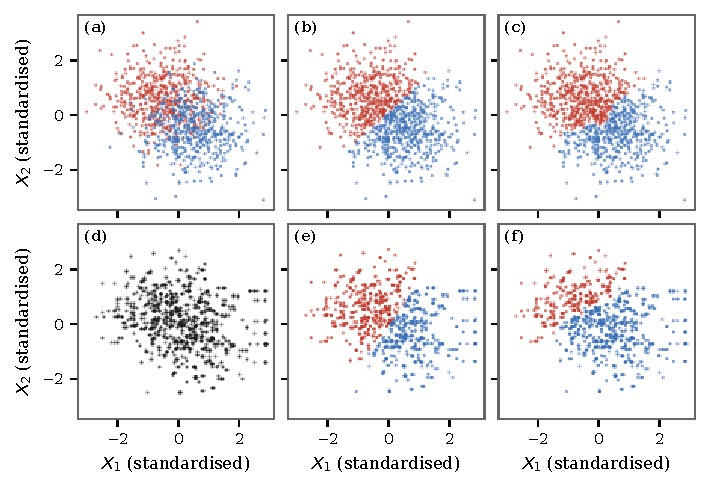
\includegraphics[width=\textwidth]{figures/fig_normal.pdf}
\caption{Normal (spherical) components: geometry largely preserved under
  synthesis. Rows are the original data (top) and one CART synthetic replicate
  (bottom); columns are the true group labels, the $k$-means partition and the
  Ward partition. In the two partition columns, colours are matched across rows
  by Hungarian alignment, so the same colour denotes corresponding groups in the
  original and synthetic panels. The lower-left panel is drawn in a single
  colour: the group label in the synthetic data is itself synthesised, so it is
  a prediction from the synthetic features rather than a planted truth, and it
  has no bijective correspondence with the original groups. Both rows contain
  the same number of observations ($N = 1000$); the synthetic panels can look
  sparser only because \DIFdelbeginFL \DIFdelFL{overlapping }\DIFdelendFL \DIFaddbeginFL \DIFaddFL{CART resamples observed values, so that }\DIFaddendFL points coincide
  more often. Scenario: $k = 2$, $p = 2$, $\rho = 0$, $\sigma = 2$.}
\label{fig:normal}
\end{figure}

\begin{figure}[t]
\centering
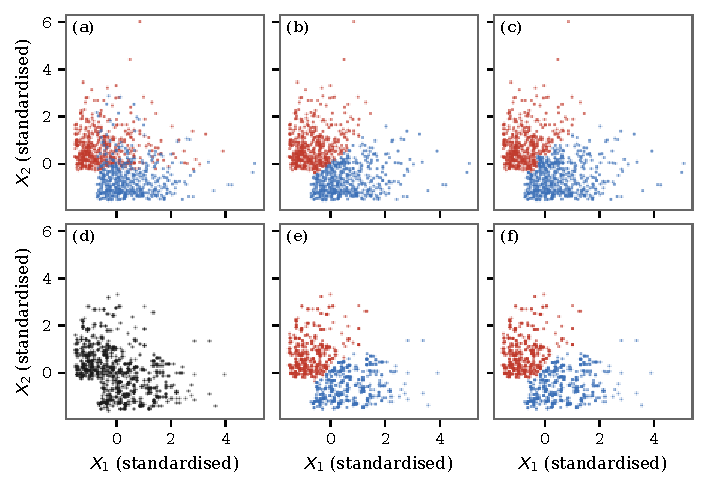
\includegraphics[width=\textwidth]{figures/fig_gamma.pdf}
\caption{Gamma (right-skewed) components: the same synthesis mechanism \DIFdelbeginFL \DIFdelFL{hardens
  }\DIFdelendFL \DIFaddbeginFL \DIFaddFL{breaks
  }\DIFaddendFL smooth tails into axis-aligned blocks. Panel layout, colour matching, the
  single-colour lower-left panel and the scenario are as in
  Fig.~\ref{fig:normal}, and both rows again contain $N = 1000$ observations.
  Comparing the lower-left panel with the upper-left one shows the \DIFdelbeginFL \DIFdelFL{artifact }\DIFdelendFL \DIFaddbeginFL \DIFaddFL{artefact
  }\DIFaddendFL directly: the continuous density gradient of the original becomes a set of
  discrete rectangular patches.}
\label{fig:gamma}
\end{figure}

\subsection{Number of groups}
\DIFaddbegin \label{sec:count}
\DIFaddend 

The number of clusters \DIFdelbegin \DIFdel{recovered }\DIFdelend \DIFaddbegin \DIFadd{estimated }\DIFaddend from synthetic data can be \DIFdelbegin \DIFdel{judged }\DIFdelend \DIFaddbegin \DIFadd{evaluated }\DIFaddend against
two references, \DIFdelbegin \DIFdel{and they answer different questions. Comparing it with the }\DIFdelend \DIFaddbegin \DIFadd{each addressing a different question
(Section~\ref{sec:metrics}). Comparison with the planted }\DIFaddend number of groups
\DIFdelbegin \DIFdel{planted by the simulation asks }\DIFdelend \DIFaddbegin \DIFadd{($\mathrm{RR}$) assesses }\DIFaddend whether the synthetic data \DIFdelbegin \DIFdel{supports
}\DIFdelend \DIFaddbegin \DIFadd{support }\DIFaddend recovery of the
underlying truth, and so \DIFdelbegin \DIFdel{confounds two failures: distortion
introduced by synthesis , and }\DIFdelend \DIFaddbegin \DIFadd{combines synthesis distortion with }\DIFaddend the inability of
the \DIFdelbegin \DIFdel{algorithm }\DIFdelend \DIFaddbegin \DIFadd{clustering procedure }\DIFaddend to find the planted structure at all. \DIFdelbegin \DIFdel{Comparing it instead }\DIFdelend \DIFaddbegin \DIFadd{Comparison }\DIFaddend with
the number \DIFdelbegin \DIFdel{a clustering algorithm
recovers from the }\emph{\DIFdel{original}} %DIFAUXCMD
\DIFdel{data }\DIFdelend \DIFaddbegin \DIFadd{estimated from the original data ($\mathrm{AG}$) }\DIFaddend isolates the
effect of synthesis\DIFdelbegin \DIFdel{, since
the same algorithm and the same estimation rule are applied on both sides. We
report both throughoutthis section, and
use the second elsewhere in the paper.
}\DIFdelend \DIFaddbegin \DIFadd{. Both are reported throughout, and
}\DIFaddend Figure~\ref{fig:recovery} shows each against separation, stratified by the true
number of groups.

Separation is the decisive factor under both references. Against the planted
\DIFdelbegin \DIFdel{truth, agreement }\DIFdelend \DIFaddbegin \DIFadd{number of groups, recovery }\DIFaddend rises from $0.272$ ($k$-means) and $0.296$ (Ward) at
$\sigma = 0.1$, through $0.304$ and $0.307$ at $\sigma = 2$, to $0.810$ and
$0.789$ at $\sigma = 6$ and $0.954$ and $0.950$ at $\sigma = 10$. The
transition is sharp: \DIFdelbegin \DIFdel{below
$\sigma \approx 2$ agreement }\DIFdelend \DIFaddbegin \DIFadd{up to $\sigma = 2$ recovery }\DIFaddend is low and dominated by the
overlap of the groups themselves, \DIFdelbegin \DIFdel{above $\sigma \approx 6$ }\DIFdelend \DIFaddbegin \DIFadd{while at $\sigma = 10$ }\DIFaddend it is near-perfect \DIFaddbegin \DIFadd{for
every $k$}\DIFaddend .

Against the \DIFdelbegin \DIFdel{partition recovered }\DIFdelend \DIFaddbegin \DIFadd{number estimated }\DIFaddend from the original data the picture is markedly
more favourable, and the gap is largest exactly where the groups overlap:
\DIFaddbegin \DIFadd{agreement is }\DIFaddend $0.751$ ($k$-means) and $0.676$ (Ward) at $\sigma = 0.1$, rising
to $0.983$ and $0.976$ at $\sigma = 10$, for overall agreement of $0.864$ and
$0.823$. The explanation is that at low separation the algorithms frequently
fail to recover the planted count from the original data as well: at
$\sigma = 0.1$, $k$-means finds the true $k$ in only $0.289$ of original
datasets and Ward in $0.306$. Much of what the first reference records as a
failure of synthesis is therefore a failure of clustering under overlap, which
synthesis reproduces faithfully. \DIFaddbegin \DIFadd{As a reference point for the size of this
agreement, two independent original datasets from the same scenario yield the
same $\hat{k}_R$ in $0.816$ ($k$-means) and $0.772$ (Ward) of pairs; a
synthetic dataset thus agrees with its parent more often than a fresh sample
from the same population would, except in the most overlapping regime
($\sigma = 0.1$), where the two are comparable for Ward and synthetic agreement
is lower for $k$-means (Supplementary Section~S4).
}\DIFaddend 

\DIFdelbegin \DIFdel{Recovery is also far easier for fewer groups . At $k = 2$ the mean recovery rate
is }\DIFdelend \DIFaddbegin \DIFadd{The number of groups behaves very differently under the two references.
Against the planted count, recovery is much higher for fewer groups: }\DIFaddend $0.843$
for $k$-means \DIFaddbegin \DIFadd{at $k = 2$}\DIFaddend , against $0.473$ at $k = 3$ and $0.439$ at $k = 4$\DIFdelbegin \DIFdel{.
The interaction is stark: }\DIFdelend \DIFaddbegin \DIFadd{;
}\DIFaddend in the overlapping regime the three- and four-group cases are almost never
recovered, yet \DIFdelbegin \DIFdel{the same cases }\DIFdelend \DIFaddbegin \DIFadd{they }\DIFaddend exceed $0.90$ once $\sigma = 10$. \DIFaddbegin \DIFadd{Against the original
data, this pattern largely disappears ($0.885$, $0.863$ and $0.844$). The
difficulty of larger $k$ thus lies mainly in the clustering problem, which
synthesis reproduces, rather than in synthesis itself. The partial $\eta^2$
values from the main-effects model make the contrast explicit: for the planted
reference, separation ($0.55$ for $k$-means, $0.57$ for Ward) and $k$ ($0.31$
and $0.37$) dominate, whereas for agreement with the original data separation
($0.20$ and $0.21$) is followed by correlation ($0.10$ and $0.07$) and
distribution family ($0.03$ and $0.10$), with $k$ below $0.01$.
}\DIFaddend Table~\ref{tab:factors} reports the marginal means for every design factor
\DIFdelbegin \DIFdel{. Dimensionality and correlation are secondary, }\DIFdelend \DIFaddbegin \DIFadd{under both references.
}

\DIFadd{Two further patterns in Table~\ref{tab:factors} deserve comment. Agreement
with the original data is higher for correlated components ($0.929$ versus
$0.800$ for $k$-means) and does not decline with dimensionality. The second of
these should not be read as evidence that synthesis is easier in higher
dimensions: at $p = 10$ }\DIFaddend and \DIFdelbegin \DIFdel{the
}\DIFdelend \DIFaddbegin \DIFadd{$\sigma \le 2$ the silhouette criterion selects
$\hat{k}_R = 2$ for $87$--$90\%$ of original datasets ($k$-means), so original
and synthetic estimates coincide largely because both collapse onto the
smallest candidate. The }\DIFaddend distribution family produces a consistent \DIFdelbegin \DIFdel{but modest gap that
}\DIFdelend \DIFaddbegin \DIFadd{gap under
both references, which }\DIFaddend Section~\ref{sec:distribution} examines\DIFdelbegin \DIFdel{directly}\DIFdelend .

\begin{figure}[t]
\centering
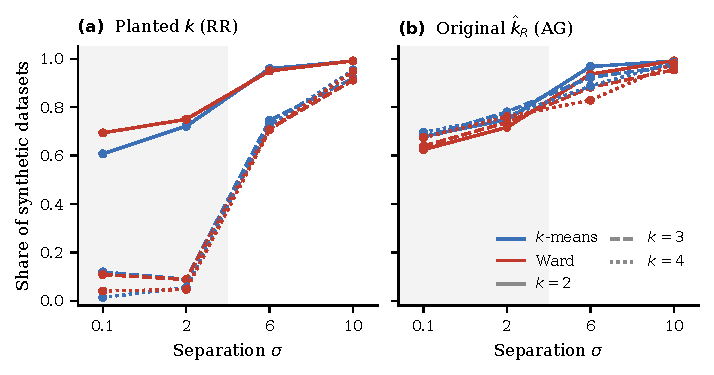
\includegraphics[width=\textwidth]{figures/fig_recovery.pdf}
\caption{Cluster-count agreement between synthetic and original data, against
  separation and stratified by the true \DIFdelbeginFL \DIFdelFL{group count}\DIFdelendFL \DIFaddbeginFL \DIFaddFL{number of groups}\DIFaddendFL , under two reference
  conventions. (a) Agreement with the number of groups planted by the
  simulation \DIFaddbeginFL \DIFaddFL{($\mathrm{RR}$)}\DIFaddendFL . (b) Agreement with the number a clustering
  algorithm recovers from the original data \DIFaddbeginFL \DIFaddFL{($\mathrm{AG}$)}\DIFaddendFL . \DIFdelbeginFL \DIFdelFL{Panel }\DIFdelendFL \DIFaddbeginFL \DIFaddFL{In panel }\DIFaddendFL (a)\DIFaddbeginFL \DIFaddFL{,
  agreement }\DIFaddendFL is \DIFdelbeginFL \DIFdelFL{flat and }\DIFdelendFL low while the groups overlap (shaded) \DIFdelbeginFL \DIFdelFL{, and collapses almost completely }\DIFdelendFL for $k \ge 3$ \DIFaddbeginFL \DIFaddFL{and
  moderate for $k = 2$}\DIFaddendFL ; panel (b) stays high throughout and depends far less on
  $k$, because in the overlapping regime the algorithms often fail to recover
  the planted count from the original data \DIFdelbeginFL \DIFdelFL{either}\DIFdelendFL \DIFaddbeginFL \DIFaddFL{as well}\DIFaddendFL , so both sides of the
  comparison \DIFdelbeginFL \DIFdelFL{are wrong }\DIFdelendFL \DIFaddbeginFL \DIFaddFL{deviate from the truth }\DIFaddendFL in the same way. The two algorithms track
  each other closely under (a) and separate \DIFdelbeginFL \DIFdelFL{slightly }\DIFdelendFL under (b). Both panels use all
  $720{,}000$ original--synthetic pairs\DIFdelbeginFL \DIFdelFL{; the unit of
  replication is the pair}\DIFdelendFL .}
\label{fig:recovery}
\end{figure}

\begin{table}[t]
\centering
\caption{\DIFdelbeginFL \DIFdelFL{Mean recovery rate of }\DIFdelendFL \DIFaddbeginFL \DIFaddFL{Agreement in }\DIFaddendFL the \DIFdelbeginFL \DIFdelFL{true }\DIFdelendFL number of groups by design factor, over the full
         720{,}000-evaluation design\DIFaddbeginFL \DIFaddFL{, under the two references of
         Eq.~\eqref{eq:sr}: the planted number of groups ($\mathrm{RR}$) and
         the number estimated from the original data ($\mathrm{AG}$). Each
         entry is a marginal mean over all other factors. Candidate range
         $\{2,\dots,\min(k+3,8)\}$; the fixed-range analysis is in
         Supplementary Table~S2}\DIFaddendFL .}
\label{tab:factors}
\small
\DIFdelbeginFL %DIFDELCMD < \begin{tabular}{llrr}
%DIFDELCMD < \toprule
%DIFDELCMD < Factor & Level & $k$-means & Ward \\
%DIFDELCMD < \midrule
%DIFDELCMD < Separation $\sigma$ & $0.1$   & 0.272 & 0.296 \\
%DIFDELCMD <                     & $2$     & 0.304 & 0.307 \\
%DIFDELCMD <                     & $6$     & 0.810 & 0.789 \\
%DIFDELCMD <                     & $10$    & 0.954 & 0.950 \\
%DIFDELCMD < \addlinespace
%DIFDELCMD < Number of groups $k$ & $2$    & 0.843 & 0.860 \\
%DIFDELCMD <                      & $3$    & 0.473 & 0.459 \\
%DIFDELCMD <                      & $4$    & 0.439 & 0.437 \\
%DIFDELCMD < \addlinespace
%DIFDELCMD < Dimensionality $p$ & $2$      & 0.616 & 0.623 \\
%DIFDELCMD <                    & $5$      & 0.561 & 0.569 \\
%DIFDELCMD <                    & $10$     & 0.578 & 0.564 \\
%DIFDELCMD < \addlinespace
%DIFDELCMD < Correlation $\rho$ & $0$      & 0.571 & 0.578 \\
%DIFDELCMD <                    & $0.4$    & 0.599 & 0.592 \\
%DIFDELCMD < \addlinespace
%DIFDELCMD < Distribution & Normal         & 0.604 & 0.610 \\
%DIFDELCMD <              & Gamma          & 0.565 & 0.561 \\
%DIFDELCMD < \midrule
%DIFDELCMD < Overall & & 0.585 & 0.585 \\
%DIFDELCMD < \bottomrule
%DIFDELCMD < \end{tabular}
%DIFDELCMD < %%%
\DIFdelendFL \DIFaddbeginFL \begin{tabular}{llrrrr}
\toprule
 & & \multicolumn{2}{c}{Planted $k$ (RR)} & \multicolumn{2}{c}{Original $\hat{k}_R$ (AG)} \\
\cmidrule(lr){3-4}\cmidrule(lr){5-6}
Factor & Level & $k$-means & Ward & $k$-means & Ward \\
\midrule
Separation $\sigma$ & $0.1$   & 0.272 & 0.296 & 0.751 & 0.676 \\
                    & $2$     & 0.304 & 0.307 & 0.797 & 0.759 \\
                    & $6$     & 0.810 & 0.789 & 0.926 & 0.882 \\
                    & $10$    & 0.954 & 0.950 & 0.983 & 0.976 \\
\addlinespace
Number of groups $k$ & $2$    & 0.843 & 0.860 & 0.885 & 0.841 \\
                     & $3$    & 0.473 & 0.459 & 0.863 & 0.812 \\
                     & $4$    & 0.439 & 0.437 & 0.844 & 0.816 \\
\addlinespace
Dimensionality $p$ & $2$      & 0.616 & 0.623 & 0.843 & 0.770 \\
                   & $5$      & 0.561 & 0.569 & 0.866 & 0.819 \\
                   & $10$     & 0.578 & 0.564 & 0.884 & 0.880 \\
\addlinespace
Correlation $\rho$ & $0$      & 0.571 & 0.578 & 0.800 & 0.763 \\
                   & $0.4$    & 0.599 & 0.592 & 0.929 & 0.884 \\
\addlinespace
Distribution $F$ & Normal     & 0.604 & 0.610 & 0.896 & 0.898 \\
                 & Gamma      & 0.565 & 0.561 & 0.833 & 0.749 \\
\midrule
Overall & & 0.585 & 0.585 & 0.864 & 0.823 \\
\bottomrule
\end{tabular}
\DIFaddendFL \end{table}

\subsection{Geometric fidelity}

Figure~\ref{fig:fidelity} traces \DIFdelbegin \DIFdel{the two }\DIFdelend \DIFaddbegin \DIFadd{two of the }\DIFaddend geometric-fidelity metrics against
separation. Mean centroid distance falls steeply as groups separate, from
$0.60$ ($k$-means) and $0.86$ (Ward) at $\sigma = 0.1$ to $0.09$ and $0.10$ at
$\sigma = 10$, because well-separated groups pin their centroids robustly
regardless of the local block \DIFdelbegin \DIFdel{artifact}\DIFdelend \DIFaddbegin \DIFadd{artefact}\DIFaddend . Mean variance difference \DIFdelbegin \DIFdel{declines in
parallel}\DIFdelend \DIFaddbegin \DIFadd{also
declines, more gradually}\DIFaddend , from $0.35$ and $0.61$ to $0.11$ and $0.13$. \DIFdelbegin \DIFdel{At every separation level and on }\DIFdelend \DIFaddbegin \DIFadd{Across
all separation levels and for }\DIFaddend both metrics, $k$-means \DIFdelbegin \DIFdel{sits }\DIFdelend \DIFaddbegin \DIFadd{lies }\DIFaddend below Ward: \DIFdelbegin \DIFdel{its centroid averaging
makes it }\DIFdelend \DIFaddbegin \DIFadd{it is
}\DIFaddend the geometrically more conservative estimator under synthesis. \DIFaddbegin \DIFadd{Over the 144
scenarios, $k$-means has the lower MCD in 133 and the lower MVD in all 144
(paired Wilcoxon $p < 10^{-20}$ for both). }\DIFaddend The intervals overlap at
$\sigma \ge 6$, where both methods \DIFdelbegin \DIFdel{are close to the floor}\DIFdelend \DIFaddbegin \DIFadd{yield values close to zero}\DIFaddend .

\begin{figure}[t]
\centering
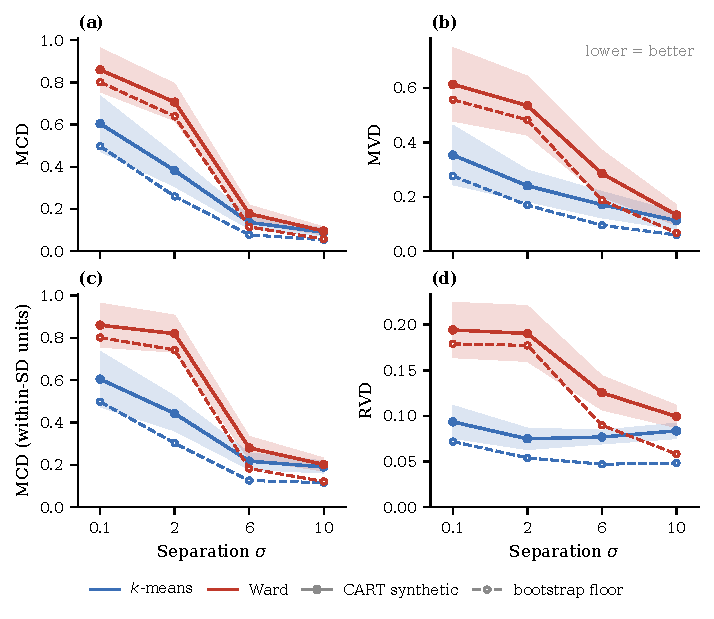
\includegraphics[width=\textwidth]{figures/fig_fidelity.pdf}
\caption{Geometric fidelity against separation. Points \DIFdelbeginFL \DIFdelFL{are means over }\DIFdelendFL \DIFaddbeginFL \DIFaddFL{show }\DIFaddendFL the \DIFdelbeginFL \DIFdelFL{144
  }\DIFdelendFL \DIFaddbeginFL \DIFaddFL{mean of the 36
  }\DIFaddendFL scenario-level means \DIFaddbeginFL \DIFaddFL{at each separation level}\DIFaddendFL ; bands are $95\%$ intervals
  computed across \DIFaddbeginFL \DIFaddFL{those }\DIFaddendFL scenarios. Left: mean centroid distance. Right: mean
  variance difference. Both \DIFaddbeginFL \DIFaddFL{panels share the vertical scale. Both metrics
  }\DIFaddendFL decline as groups separate, and $k$-means remains below Ward throughout.}
\label{fig:fidelity}
\end{figure}

\DIFdelbegin \DIFdel{Dimensionality is the strongest amplifier of variance distortion }\DIFdelend \DIFaddbegin \DIFadd{Total dispersion distortion grows with dimensionality}\DIFaddend .
Figure~\ref{fig:balance}(a) shows MVD \DIFdelbegin \DIFdel{growing steeply }\DIFdelend \DIFaddbegin \DIFadd{rising }\DIFaddend with the number of variables: for
$k$-means from $0.06$ \DIFaddbegin \DIFadd{($95\%$ interval $0.05$--$0.08$) }\DIFaddend at $p = 2$ to $0.39$
\DIFaddbegin \DIFadd{($0.32$--$0.47$) }\DIFaddend at $p = 10$, and for Ward from $0.13$ to $0.65$. \DIFdelbegin \DIFdel{Each additional synthesised dimension
compounds }\DIFdelend \DIFaddbegin \DIFadd{Because $v_j$
in Eq.~\eqref{eq:mvd} is a sum of squared deviations over the $p$ coordinates,
this growth should be read per coordinate: $\mathrm{MVD}/p$ is roughly constant
($k$-means $0.032$, $0.040$ and $0.039$ at $p = 2, 5, 10$; Ward $0.067$,
$0.078$ and $0.065$). Each synthesised coordinate therefore contributes a
similar amount of dispersion distortion, and the total accumulates with $p$ as
}\DIFaddend the axis-aligned leaf structure of Eq.~\eqref{eq:cart} \DIFdelbegin \DIFdel{. This is the
mechanism behind the mild degradation of recovery at higher }\DIFdelend \DIFaddbegin \DIFadd{is repeated in every
dimension. Unlike the count, which is protected at high }\DIFaddend $p$ \DIFdelbegin \DIFdel{in
Table~\ref{tab:factors}}\DIFdelend \DIFaddbegin \DIFadd{by the collapse of
$\hat{k}$ onto small values (Section~\ref{sec:count}), the within-cluster
dispersion is measured at the planted $k$ and so exposes this accumulation
directly}\DIFaddend .

Figure~\ref{fig:balance}(b) shows the group-balance error $\Delta G$ by
distribution family. Both algorithms preserve \DIFdelbegin \DIFdel{balance }\DIFdelend \DIFaddbegin \DIFadd{cluster sizes }\DIFaddend better on Normal
than on Gamma data ($k$-means $0.028$ versus $0.032$; Ward $0.057$ versus
$0.065$), consistent with the block \DIFdelbegin \DIFdel{artifact }\DIFdelend \DIFaddbegin \DIFadd{artefact }\DIFaddend being more disruptive on skewed
groups. More striking is that $k$-means yields systematically lower and \DIFdelbegin \DIFdel{tighter }\DIFdelend \DIFaddbegin \DIFadd{less
variable }\DIFaddend $\Delta G$ than Ward \DIFdelbegin \DIFdel{at both distributions . This reflects a structural property of the
algorithm rather than better fidelity: the within-cluster sum-of-squares
objective of Eq. ~\eqref{eq:wcss} favours partitions of comparable size, so
}\DIFdelend \DIFaddbegin \DIFadd{for both distributions (lower in 138 of 144
scenarios; overall $0.030$ versus $0.061$). Because the planted groups have
equal sizes, this difference does not reflect the preservation of a genuine
imbalance; it shows that the cluster sizes of a }\DIFaddend $k$-means \DIFdelbegin \DIFdel{tends to equalise group sizesand thereby suppresses the natural
imbalancethat skewed data would otherwise produce. Ward imposes no such
balancing pressure and follows the block-distorted density more literally,
preserving imbalance at the cost of higher variance across replicates}\DIFdelend \DIFaddbegin \DIFadd{partition fluctuate
less under synthesis}\DIFaddend . This is \DIFdelbegin \DIFdel{the clearest algorithmic difference the
study uncovers: not a difference in
accuracy, but in the kind of geometric bias each method introduces}\DIFdelend \DIFaddbegin \DIFadd{consistent with the known tendency of the
$k$-means criterion to produce clusters of similar size \mbox{%DIFAUXCMD
\citep{xiong2009}}\hskip0pt%DIFAUXCMD
.
Ward's linkage uses a related sum-of-squares criterion, but its greedy,
irreversible merges let local density irregularities created by the block
artefact move whole subsets of points between clusters. Whether $k$-means would
also understate a genuine size imbalance cannot be tested with balanced
groups, and is left to future work (Section~\ref{sec:future})}\DIFaddend .

\begin{figure}[t]
\centering
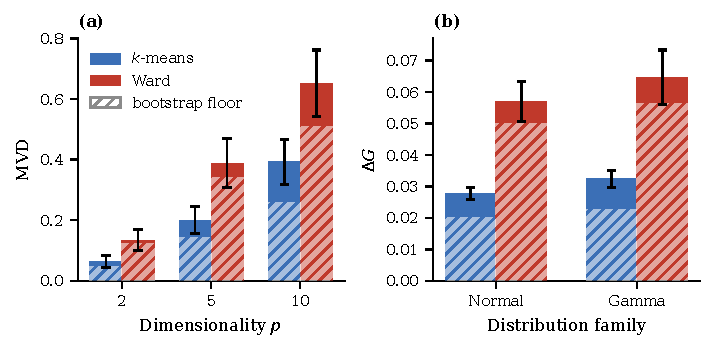
\includegraphics[width=\textwidth]{figures/fig_balance.pdf}
\caption{(a) Mean variance difference by dimensionality: \DIFaddbeginFL \DIFaddFL{total }\DIFaddendFL distortion
  \DIFdelbeginFL \DIFdelFL{grows
  steeply }\DIFdelendFL \DIFaddbeginFL \DIFaddFL{accumulates }\DIFaddendFL as dimensions are added, more so for Ward\DIFaddbeginFL \DIFaddFL{; per coordinate it is
  roughly constant (see text)}\DIFaddendFL . (b) Group-balance error
  \DIFdelbeginFL \DIFdelFL{$|\Delta G|$ }\DIFdelendFL \DIFaddbeginFL \DIFaddFL{$\Delta G$ }\DIFaddendFL by distribution family: $k$-means produces lower and \DIFdelbeginFL \DIFdelFL{tighter
  }\DIFdelendFL \DIFaddbeginFL \DIFaddFL{less variable
  }\DIFaddendFL balance error \DIFdelbeginFL \DIFdelFL{at }\DIFdelendFL \DIFaddbeginFL \DIFaddFL{for }\DIFaddendFL both distributions\DIFdelbeginFL \DIFdelFL{, reflecting the balancing pressure of its
  objective function}\DIFdelendFL . \DIFdelbeginFL \DIFdelFL{Error }\DIFdelendFL \DIFaddbeginFL \DIFaddFL{Bars are means of scenario-level means;
  error }\DIFaddendFL bars are $95\%$ intervals \DIFaddbeginFL \DIFaddFL{computed across scenarios}\DIFaddendFL .}
\label{fig:balance}
\end{figure}

\subsection{Distribution family}
\label{sec:distribution}

The distribution family is the factor that exposes the CART \DIFdelbegin \DIFdel{artifact }\DIFdelend \DIFaddbegin \DIFadd{artefact }\DIFaddend most
directly. Figure~\ref{fig:distribution} stratifies \DIFdelbegin \DIFdel{recovery }\DIFdelend \DIFaddbegin \DIFadd{count agreement }\DIFaddend by
distribution and separation \DIFdelbegin \DIFdel{. In the overlapping regime }\DIFdelend \DIFaddbegin \DIFadd{under both references, and the two panels tell
different stories. Against the planted number of groups (panel a), }\DIFaddend the two
families \DIFdelbegin \DIFdel{are indistinguishable,
because recovery is limited by the overlap rather than by synthesis. In the
informative regime the gap opens}\DIFdelend \DIFaddbegin \DIFadd{show similar recovery while the groups overlap and diverge at
intermediate separation}\DIFaddend : at $\sigma = 6$, $k$-means recovers the \DIFdelbegin \DIFdel{Normal structure }\DIFdelend \DIFaddbegin \DIFadd{planted count
}\DIFaddend $86.2\%$ of the time \DIFdelbegin \DIFdel{but the Gamma structure }\DIFdelend \DIFaddbegin \DIFadd{for Normal data but }\DIFaddend only $75.9\%$ \DIFaddbegin \DIFadd{for Gamma data }\DIFaddend (Ward:
\DIFdelbegin \DIFdel{$84.55\%$ }\DIFdelend \DIFaddbegin \DIFadd{$84.6\%$ }\DIFaddend versus $73.3\%$). \DIFdelbegin \DIFdel{By $\sigma = 10$ the gap closes again}\DIFdelend \DIFaddbegin \DIFadd{Almost all of this gap, however, is already present
in the original data, where the planted count is recovered in $90.0\%$ versus
$80.0\%$ of datasets ($k$-means; Ward $91.1\%$ versus $78.9\%$). It therefore
reflects mainly how difficult skewed groups are to cluster, not what synthesis
does to them.
}

\DIFadd{Against the original data (panel b), which isolates synthesis, the Gamma
penalty is concentrated where the groups overlap and is much larger for Ward.
At $\sigma = 0.1$, Ward's agreement is $0.806$ for Normal but only $0.545$ for
Gamma data, and at $\sigma = 2$ it is $0.878$ versus $0.639$; the
corresponding values for $k$-means are $0.765$ versus $0.737$ and $0.888$
versus $0.707$. At $\sigma = 6$ the gap narrows ($k$-means $0.947$ versus
$0.906$; Ward $0.924$ versus $0.841$), and by $\sigma = 10$ it has closed}\DIFaddend , as
separation overwhelms the \DIFdelbegin \DIFdel{artifact}\DIFdelend \DIFaddbegin \DIFadd{artefact}\DIFaddend .

This addresses the first \DIFdelbegin \DIFdel{question}\DIFdelend \DIFaddbegin \DIFadd{objective}\DIFaddend . CART preserves the \DIFdelbegin \DIFdel{signal }\DIFdelend \DIFaddbegin \DIFadd{structure }\DIFaddend needed to
recover the number of groups well on \DIFdelbegin \DIFdel{spherical }\DIFdelend Normal data, but its hardening of skewed
densities \DIFdelbegin \DIFdel{measurably reduces recovery }\DIFdelend \DIFaddbegin \DIFadd{is associated with lower agreement }\DIFaddend on Gamma data\DIFdelbegin \DIFdel{across precisely the range
of separations where recovery is otherwise achievable}\DIFdelend \DIFaddbegin \DIFadd{, most markedly when
groups are not well separated and for the hierarchical method}\DIFaddend .

\begin{figure}[t]
\centering
\DIFdelbeginFL %DIFDELCMD < 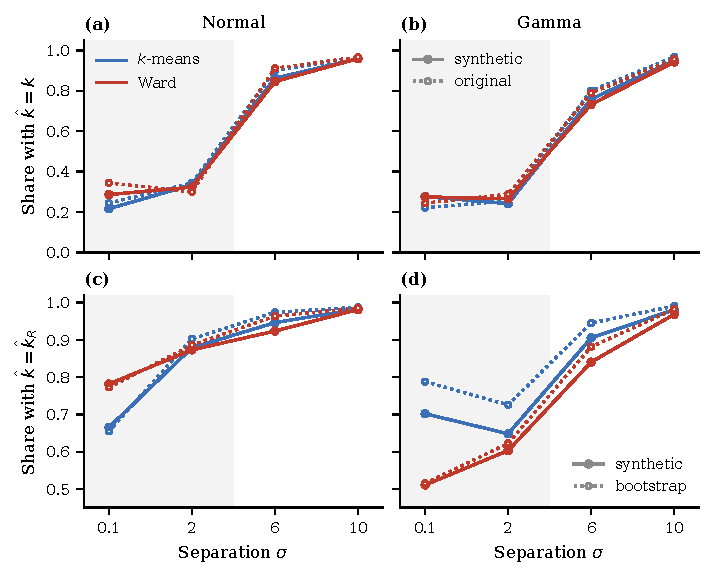
\includegraphics[width=0.62\textwidth]{figures/fig_distribution.pdf}
%DIFDELCMD < %%%
\DIFdelendFL \DIFaddbeginFL 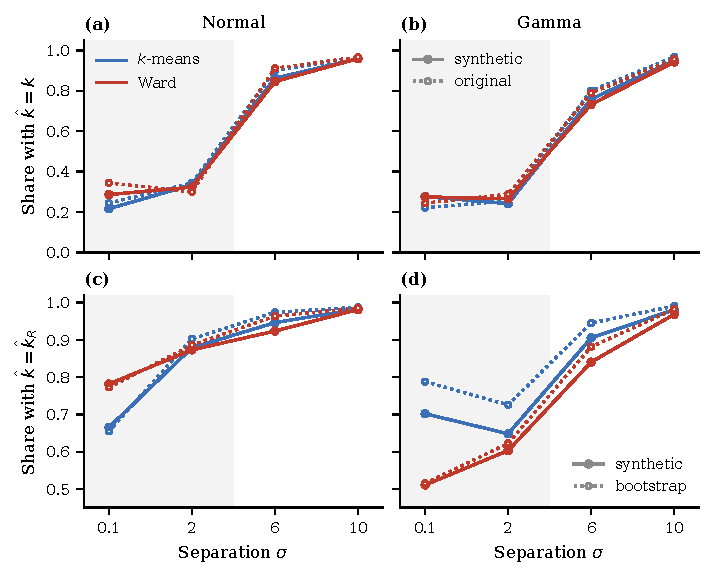
\includegraphics[width=\textwidth]{figures/fig_distribution.pdf}
\DIFaddendFL \caption{\DIFdelbeginFL \DIFdelFL{Recovery of the number of groups }\DIFdelendFL \DIFaddbeginFL \DIFaddFL{Cluster-count agreement }\DIFaddendFL by distribution family and separation\DIFaddbeginFL \DIFaddFL{, under
  the two references}\DIFaddendFL . \DIFdelbeginFL \DIFdelFL{The }\DIFdelendFL \DIFaddbeginFL \DIFaddFL{(a) Versus the planted number of groups: the two
  }\DIFaddendFL families \DIFdelbeginFL \DIFdelFL{are indistinguishable }\DIFdelendFL \DIFaddbeginFL \DIFaddFL{show similar recovery }\DIFaddendFL while groups overlap and diverge \DIFdelbeginFL \DIFdelFL{in the informative regime}\DIFdelendFL \DIFaddbeginFL \DIFaddFL{at
  intermediate separation}\DIFaddendFL , where \DIFaddbeginFL \DIFaddFL{recovery is lower for }\DIFaddendFL Gamma data \DIFdelbeginFL \DIFdelFL{depresses recovery }\DIFdelendFL for both
  algorithms. \DIFaddbeginFL \DIFaddFL{(b) Versus the number recovered from the original data: the
  Gamma penalty attributable to synthesis is largest in the overlapping regime
  and for Ward.}\DIFaddendFL }
\label{fig:distribution}
\end{figure}

\subsection{Agreement between the two algorithms}
%DIF <  Reviewer note (Jordi, p14): this comparison reads better as the last
%DIF <  results subsection than as the third.

Whether the two \DIFdelbegin \DIFdel{paradigms }\DIFdelend \DIFaddbegin \DIFadd{methods }\DIFaddend differ in robustness to synthetic distortion was the
third \DIFdelbegin \DIFdel{question. They do not, at least not on recovery. The overall recovery rates are
$0.585$ ($k$-means) and }\DIFdelend \DIFaddbegin \DIFadd{objective, and the answer depends on the reference. Against the planted
number of groups the two are indistinguishable: overall recovery is }\DIFaddend $0.585$
\DIFdelbegin \DIFdel{(Ward); }\DIFdelend \DIFaddbegin \DIFadd{for both, }\DIFaddend a paired Wilcoxon signed-rank test across the 144 scenario-level
means finds no significant difference (\DIFdelbegin \DIFdel{$W = 3300.0$}\DIFdelend \DIFaddbegin \DIFadd{$W = 3300$}\DIFaddend , $p = 0.39$), and the two
algorithms \DIFdelbegin \DIFdel{agree on the }\DIFdelend \DIFaddbegin \DIFadd{reach the same }\DIFaddend outcome in $92.0\%$ of individual evaluations.
\DIFdelbegin \DIFdel{The hypothesis that connectivity-based
clustering would be
materially more robust (plausible given its ability to
follow non-convex structure) }\DIFdelend \DIFaddbegin \DIFadd{Against the original data, which isolates synthesis, $k$-means is more stable:
overall agreement is $0.864$ versus $0.823$, $k$-means is higher in 95 of the
144 scenarios (24 ties), and the paired test is significant ($W = 1665$,
$p < 0.001$). The conclusion is unchanged under the fixed candidate range
(Supplementary Section~S3). Together with the geometric results, this
indicates that $k$-means is the more robust of the two methods to CART
synthesis, whereas the prior expectation that a hierarchical method would be
more robust }\DIFaddend is not supported.

As a complementary check on internal cohesion, the difference in mean
silhouette width between synthetic and original partitions is small and
centred near zero at every separation \DIFaddbegin \DIFadd{(within $\pm 0.012$)}\DIFaddend . The absolute
levels are nearly identical ($k$-means $0.396$ versus $0.397$; Ward $0.376$
versus $0.377$), \DIFdelbegin \DIFdel{confirming that CART neither manufactures nor destroys apparent cluster quality }\DIFdelend \DIFaddbegin \DIFadd{suggesting that the apparent clustering quality is similar
before and after synthesis}\DIFaddend . This is reassuring, but it also means that
silhouette alone would fail to flag the geometric distortions the other
metrics detect, an instructive negative result for anyone tempted to validate
a synthetic release with an internal index.

% =====================================================================
\section{Discussion}
%DIF <  Reviewer note (Jordi + Dani, p18): "Discussion" rather than "Conclusions".
% =====================================================================

This study evaluated whether CART-generated synthetic data \DIFdelbegin \DIFdel{preserves }\DIFdelend \DIFaddbegin \DIFadd{preserve }\DIFaddend the
structural properties that cluster analysis relies on, comparing $k$-means and
Ward's hierarchical clustering across a 144-scenario factorial design and
720{,}000 synthetic-versus-original evaluations. Four findings emerge.

First, separation dominates \DIFdelbegin \DIFdel{recovery of }\DIFdelend \DIFaddbegin \DIFadd{agreement in }\DIFaddend the number of groups. \DIFdelbegin \DIFdel{The recovery rate
}\DIFdelend \DIFaddbegin \DIFadd{Agreement with
the original data rises from $0.75$ ($k$-means) when the groups overlap to
$0.98$ when they are well separated, and recovery of the planted count }\DIFaddend rises
from roughly $0.27$ \DIFdelbegin \DIFdel{in the overlapping regime }\DIFdelend to above $0.95$\DIFdelbegin \DIFdel{at
$\sigma = 10$, with the }\DIFdelend \DIFaddbegin \DIFadd{. The }\DIFaddend number of groups \DIFdelbegin \DIFdel{the second factor: easy }\DIFdelend \DIFaddbegin \DIFadd{strongly affects
recovery of the planted count (higher }\DIFaddend at $k = 2$\DIFdelbegin \DIFdel{(}\DIFdelend \DIFaddbegin \DIFadd{, }\DIFaddend $0.84$\DIFdelbegin \DIFdel{) and hard }\DIFdelend \DIFaddbegin \DIFadd{, and lower }\DIFaddend at
$k \ge 3$\DIFdelbegin \DIFdel{(}\DIFdelend \DIFaddbegin \DIFadd{, }\DIFaddend below $0.48$) \DIFdelbegin \DIFdel{. Dimensionality, correlation and distribution family act as secondary modulators. A practical implication is
that a synthetic release is most trustworthy for clustering exactly where
clustering is easiest, and least trustworthy where the analyst most needs help}\DIFdelend \DIFaddbegin \DIFadd{but has little effect on agreement between original
and synthetic estimates. Overall, recovery is highest for simpler cluster
structures, with well-separated and fewer groups, and lowest for more complex
structures, with overlap and a larger number of groups; most of the effect of
$k$, however, is a property of the clustering problem that synthesis
reproduces rather than a distortion that synthesis introduces}\DIFaddend .

Second, \DIFaddbegin \DIFadd{we found no significant difference between }\DIFaddend the two algorithms \DIFdelbegin \DIFdel{are statistically indistinguishable on recovery }\DIFdelend \DIFaddbegin \DIFadd{in
recovery of the planted count }\DIFaddend ($0.585$ versus $0.585$; $p = 0.39$\DIFdelbegin \DIFdel{; $92\%$ agreement). Where they differ is in
the geometric bias they introduce. }\DIFdelend \DIFaddbegin \DIFadd{), but
}\DIFaddend $k$-means is the more \DIFdelbegin \DIFdel{conservative
estimator (}\DIFdelend \DIFaddbegin \DIFadd{stable of the two when synthetic estimates are compared
with those from the original data ($0.864$ versus $0.823$; $p < 0.001$). The
same ordering holds for the geometry: $k$-means shows }\DIFaddend lower centroid and
variance distortion at every separation \DIFdelbegin \DIFdel{), and its objective imposes a balancing bias that suppresses group-size imbalance.
Ward preserves imbalance more faithfully but with higher variance}\DIFdelend \DIFaddbegin \DIFadd{and smaller fluctuations in cluster
sizes}\DIFaddend . For an applied analyst\DIFdelbegin \DIFdel{this is the more actionable result than the null on accuracy :
if group sizes are themselves a finding}\DIFdelend \DIFaddbegin \DIFadd{, the practical implication is that the choice of
algorithm matters more for the fidelity of a synthetic-data analysis than
accuracy against a ground truth would suggest. It also raises a question that
this design cannot answer: because the $k$-means criterion favours clusters of
similar size}\DIFaddend , a $k$-means analysis of synthetic data \DIFdelbegin \DIFdel{will understate imbalance in a way that is invisible from the partition alone}\DIFdelend \DIFaddbegin \DIFadd{may understate a genuine
imbalance, which only a design with unequal group sizes can test}\DIFaddend .

Third, CART is not utility-neutral, and its \DIFdelbegin \DIFdel{failure mode is distributional. On spherical }\DIFdelend \DIFaddbegin \DIFadd{performance depends on the
underlying distribution. On }\DIFaddend Normal data it is close to neutral; on skewed
Gamma data it hardens smooth density gradients into axis-aligned blocks,
visibly distorting geometry and \DIFdelbegin \DIFdel{measurably depressing recovery in the informative regime. Degradation }\DIFdelend \DIFaddbegin \DIFadd{being associated with lower agreement,
particularly for Ward's linkage and when groups overlap. Total dispersion
distortion }\DIFaddend grows with dimensionality, \DIFdelbegin \DIFdel{as each synthesised dimension compounds the block
structure}\DIFdelend \DIFaddbegin \DIFadd{because each synthesised coordinate
contributes a similar amount of distortion}\DIFaddend .

Fourth, and methodologically, an internal validity index is not a sufficient
check. Silhouette \DIFdelbegin \DIFdel{geometry is preserved almost exactly }\DIFdelend \DIFaddbegin \DIFadd{values remain almost unchanged }\DIFaddend even where centroid and
dispersion fidelity degrade substantially. A practitioner who validates a
synthetic release by confirming that its silhouette profile matches the
original \DIFdelbegin \DIFdel{will }\DIFdelend \DIFaddbegin \DIFadd{may }\DIFaddend conclude that structure is intact in precisely the settings where
this analysis shows it is not. \DIFaddbegin \DIFadd{A related methodological point concerns the
reference: the planted truth, the natural choice in a simulation, answers a
different question from the one a data holder faces, and in this study it
masked the difference between the two algorithms.
}\DIFaddend 

An interesting corollary of the design is that clustering can be read in the
other direction, as an instrument rather than an object of study. Because a
partition responds to local density, separability and dispersion
simultaneously, the agreement between partitions recovered from original and
synthetic data functions as a sensitive summary of geometric resemblance, one
that reacts to distortions which marginal and bivariate checks \DIFdelbegin \DIFdel{do not see}\DIFdelend \DIFaddbegin \DIFadd{may not detect}\DIFaddend .
We did not pursue this here, but the metrics of Section~\ref{sec:metrics} could
be repurposed as general-utility diagnostics rather than task-specific ones.

\subsection{Relation to previous work}

The study extends \citet{chen2025} in three ways: a structurally distinct
second algorithm, a skewed distribution family that exposes tree-synthesis
\DIFdelbegin \DIFdel{artifacts, and ground-truth-referenced }\DIFdelend \DIFaddbegin \DIFadd{artefacts, and }\DIFaddend structural metrics that \DIFdelbegin \DIFdel{do not depend on
the
synthetic data alone}\DIFdelend \DIFaddbegin \DIFadd{compare partitions recovered from the
original and synthetic data}\DIFaddend . The conclusion that CART is a reasonable default
for well-behaved data but degrades on skewed distributions is consistent with
the broader \texttt{synthpop} literature \citep{nowok2016,snoke2018}, and the
qualitative block \DIFdelbegin \DIFdel{artifact }\DIFdelend \DIFaddbegin \DIFadd{artefact }\DIFaddend matches the known axis-aligned bias of sequential
tree synthesis. The finding that utility rankings depend on the downstream task
echoes benchmarking work in the health-records setting
\citep{yan2022,elemam2022}, where the same generator changes position depending
on which analysis is used to score it\DIFaddbegin \DIFadd{, and an applied study of wearable
physiological data in mental-health monitoring similarly found that the
clustering utility of }\texttt{\DIFadd{synthpop}} \DIFadd{releases depends on the synthesis
settings \mbox{%DIFAUXCMD
\citep{vidiella2025}}\hskip0pt%DIFAUXCMD
. The greater sensitivity of Ward's linkage to
perturbation of the data is in line with the classical robustness comparisons
of \mbox{%DIFAUXCMD
\citet{milligan1980}}\hskip0pt%DIFAUXCMD
}\DIFaddend . A parallel question arises when values are missing
rather than synthesised: \citet{aschenbruck2023} evaluate how imputation
strategies affect the clusters subsequently recovered from mixed-type data, and
reach a structurally similar conclusion, that the imputation model and the
clustering method interact and cannot be assessed in isolation. Since CART
underlies both sequential synthesis and widely used non-parametric imputation,
the two literatures are closer than their vocabularies suggest.

\subsection{Limitations}
\label{sec:limitations}

The evaluation uses controlled simulations with known ground truth rather than
real \DIFdelbegin \DIFdel{administrative }\DIFdelend data. This isolates mechanisms cleanly but limits direct generalisation to
\DIFdelbegin \DIFdel{messy }\DIFdelend data with missingness, mixed types\DIFaddbegin \DIFadd{, unequal group sizes }\DIFaddend and unknown
data-generating processes. The generator is limited to CART \DIFaddbegin \DIFadd{with a single
parameterisation (minimum leaf size ten, fixed variable order) }\DIFaddend and the
algorithms to $k$-means and Ward; density-based and model-based clustering,
\DIFaddbegin \DIFadd{other synthesis settings, }\DIFaddend and parametric or deep generative synthesisers, may
behave differently. Sample size was fixed at $N = 1000$, so small-sample
behaviour is unexamined\DIFdelbegin \DIFdel{, and the geometric-fidelity metrics were computed on a balanced subset of the synthetic
draws rather than all of them}\DIFdelend \DIFaddbegin \DIFadd{. The number of groups is selected by the silhouette
criterion over $\hat{k} \ge 2$, so a single-cluster solution can never be
chosen, even when the groups overlap so strongly that one cluster is the most
reasonable description; other selection rules \mbox{%DIFAUXCMD
\citep{milligan1985} }\hskip0pt%DIFAUXCMD
may
respond differently to synthesis. Finally, count agreement is inflated where
the estimator collapses onto a small number of candidate values, as happens at
high $p$ and low $\sigma$, and should be read together with the geometric
metrics}\DIFaddend .

Two conventions in the definition of MCD and MVD deserve emphasis, because both
affect the numbers themselves and not only their interpretation. The first is
what the metrics compare. Here they compare the partition recovered from the
original data against the partition recovered from the synthetic data, which is
the quantity a claim about synthesis requires; the superficially similar
practice of comparing a recovered partition against the planted labels of the
same dataset measures clustering accuracy instead, and carries no information
about the generator. The second is scale. Both metrics are computed after
standardising with a scaler fit on the original data and applied unchanged to
the synthetic data, so both are expressed in units of the original feature
scale. Standardising each dataset separately rescales away part of the
distortion the metrics are meant to capture, and omitting standardisation
altogether makes MVD track absolute cluster spread (which grows with $\sigma$
by construction), so that the metric rises with separation when what it is
measuring is the design parameter. Absolute values of MCD and MVD are therefore
not comparable across studies that differ in either convention, and any
replication should state both explicitly. \DIFaddbegin \DIFadd{Both metrics are also unnormalised sums over
coordinates, so their absolute values grow with $p$ even at constant
per-coordinate distortion; comparisons across dimensionality should use
per-coordinate or relative versions.
}\DIFaddend 

\subsection{Future work}
\DIFaddbegin \label{sec:future}
\DIFaddend 

The central lesson generalises beyond the specific methods studied: synthetic
data utility is task-relative, and a generator that preserves marginal
resemblance need not preserve the higher-order geometry a clustering workflow
depends on. Practically, the results argue for validating structural fidelity
(distances, dispersion, separability, balance) against the intended analysis,
and for treating a clustering comparison as \DIFdelbegin \DIFdel{the }\DIFdelend \DIFaddbegin \DIFadd{a }\DIFaddend more demanding resemblance check
\DIFdelbegin \DIFdel{that marginal summaries cannot }\DIFdelend \DIFaddbegin \DIFadd{than marginal summaries can }\DIFaddend provide. Natural extensions include other
synthesisers (parametric mixtures, copulas, deep generative models) \DIFaddbegin \DIFadd{and other
CART settings}\DIFaddend , non-convex and density-based clustering, \DIFaddbegin \DIFadd{unequal group sizes,
}\DIFaddend varying $N$ to probe small-sample behaviour, and \DIFdelbegin \DIFdel{real datasets with established latent structure}\DIFdelend \DIFaddbegin \DIFadd{chance-corrected partition
comparisons such as the adjusted Rand index \mbox{%DIFAUXCMD
\citep{hubert1985} }\hskip0pt%DIFAUXCMD
computed on a
common set of points}\DIFaddend . A promising direction is to model the discrepancy
$\Delta$ of Eq.~\eqref{eq:discrepancy} directly as a learned function of the
design factors, turning the utility surface itself into a predictive tool.

\DIFdelbegin \subsection*{\DIFdel{Code availability}}
%DIFAUXCMD
%DIFDELCMD < 

%DIFDELCMD < %%%
\DIFdel{The full pipeline, from data generation through to the figures and tables
reported here, is available at
}%DIFDELCMD < \url{https://github.com/Sterrysx/synthetic-clustering}%%%
\DIFdel{. Every stage is driven
from a single configuration file and can be re-executed end to end}\DIFdelend \DIFaddbegin \DIFadd{As a concrete next step, we propose applying the framework to the wearable
dataset described in \mbox{%DIFAUXCMD
\citet{vidiella2025}}\hskip0pt%DIFAUXCMD
, to which we have direct access.
Beyond providing a real-data test of the present design, this dataset would
allow a comparison that neither study can perform alone. The present work
evaluates synthesis as substitution, in which the synthetic dataset replaces
the original. The applied study instead evaluates augmentation, in which the
synthetic records are appended to the real ones and the union is clustered.
These are different operations, and their effects are currently confounded
with sample size: doubling the number of observations alters neighbourhood
parameters and silhouette values independently of any distortion introduced by
the generator. A three-way comparison of the partitions recovered from the real
data, from the synthetic data alone, and from the augmented set, evaluated with
the same metrics used here, would separate the effect of the generator from
the effect of the additional sample. It would also make it possible to test
whether the parameterisation of the generator, rather than the generator
itself, accounts for the block artefact documented in this paper, since the
applied study reports a substantial improvement in utility after replacing
CART with conditional inference trees \mbox{%DIFAUXCMD
\citep{hothorn2006} }\hskip0pt%DIFAUXCMD
and increasing the
minimum leaf size. We regard this comparison as a natural continuation of the
present study and as a practical way of establishing which of its conclusions
generalise beyond the simulated setting.
}

%DIF >  =====================================================================
\section{Conclusions}
%DIF >  =====================================================================

\DIFadd{In our view, the main contribution of this study is that its discrepancy
framework does not depend on the simulation that illustrates it. The quantity
$\Delta(\theta_R, \theta_S)$ is defined for any reference dataset and any
generator, and the five factors varied here all have direct empirical
counterparts: separation corresponds to how distinct the underlying groups
are, the number of groups to the number of latent subpopulations,
dimensionality to the number of recorded variables, correlation to the
dependence between features, and the distribution family to the shape of the
observed densities. The simulation fixes these factors by construction, but in
an applied dataset they can be measured. This means the framework can be
transferred to real data without modification, and we believe such a transfer
would be informative rather than merely confirmatory. Real datasets occupy
regions of the design space that the present grid does not reach. Behavioural
and physiological measurements routinely show correlations above $0.95$
between related features, well beyond the maximum of $\rho = 0.4$ examined
here, and skewness values considerably higher than those produced by the Gamma
family. They also exhibit properties the simulation excludes altogether, such
as strongly unbalanced group sizes, ambiguous missingness in which a zero may
indicate either genuine inactivity or a non-worn device, and heterogeneity
between individuals. Each of these is a plausible source of additional
distortion under sequential tree synthesis, and each would help to refine the
conclusions reported here. We consider the unbalanced case particularly
relevant, because the group-balance error $\Delta G$ and the hypothesis that
the $k$-means criterion understates imbalance can only be fully tested when a
substantial imbalance is present in the reference data}\DIFaddend .

\DIFdelbegin \DIFdel{Synthetic }\DIFdelend \DIFaddbegin \DIFadd{Within the region of the design space studied here, synthetic }\DIFaddend data generated
with CART can reproduce the appearance of clustering structure while subtly
reshaping its geometry. Both algorithms recover well-separated structure
reliably and \DIFdelbegin \DIFdel{fail }\DIFdelend \DIFaddbegin \DIFadd{struggle }\DIFaddend together when groups overlap; where they diverge is in
\DIFdelbegin \DIFdel{the }\DIFdelend \DIFaddbegin \DIFadd{how faithfully each reproduces, on synthetic data, the partition it would have
found on the original data, and in the geometric }\DIFaddend bias each imprints on the
recovered partition. The utility of synthetic data for clustering is therefore
best understood not as a property of the data but as a property of the
data--generator--algorithm triple, to be verified rather than assumed.

\DIFaddbegin \backmatter

\bmhead{Supplementary information}
\DIFadd{The online supplementary material contains the recovery heatmap by number of
groups and separation, the contingency table of original versus synthetic
estimates, the sensitivity analysis for the candidate range of $\hat{k}$, and
the independent-resampling baseline.
}

\section*{\DIFadd{Declarations}}

\noindent \textbf{\DIFadd{Funding:}} [\DIFadd{To be completed by the authors.}]

\noindent \textbf{\DIFadd{Competing interests:}} [\DIFadd{To be completed by the authors.}]

\noindent \textbf{\DIFadd{Data availability:}} \DIFadd{All data analysed in this study are
  simulated; they can be regenerated exactly from the configuration file and
  seeds distributed with the code.
}

\noindent \textbf{\DIFadd{Code availability:}} \DIFadd{The full pipeline, from data generation
  through to the figures and tables reported here, is available at
  }\url{https://github.com/Sterrysx/synthetic-clustering}\DIFadd{. Every stage is driven
  from a single configuration file and can be re-executed end to end.
}

\noindent \textbf{\DIFadd{Author contributions:}} [\DIFadd{To be completed by the authors.}]

\bibliography{refs}

\DIFaddend \begin{appendices}

\section{Clustering objectives}
\label{app:algorithms}

$k$-means partitions $N$ observations $\{x_i\}_{i=1}^N$, $x_i \in
\mathbb{R}^p$, into $k$ non-overlapping groups by minimising the within-cluster
sum of squares \citep{macqueen1967}. Writing $\mathcal{C} = \{C_1,\dots,C_k\}$
for the partition and $\mu_j$ for the centroid of $C_j$,
\begin{equation}
  \arg\min_{\mathcal{C}} \sum_{j=1}^{k} \sum_{x_i \in C_j}
    \lVert x_i - \mu_j \rVert^2,
  \qquad
  \mu_j = \frac{1}{|C_j|}\sum_{x_i \in C_j} x_i .
  \label{eq:wcss}
\end{equation}
Lloyd's iteration alternates assignment and update steps until the partition
stabilises, converging to a local optimum.

Hierarchical clustering builds a dendrogram by successive merging
\citep{ward1963}. Each observation begins as a singleton; at every step the two
clusters whose merger least increases the total within-cluster error sum of
squares are combined. With
\begin{equation}
  \mathrm{ESS} = \sum_j \sum_{x_i \in C_j} \lVert x_i - \mu_j \rVert^2,
  \qquad
  \Delta_{\text{Ward}}(C_a, C_b)
    = \frac{|C_a|\,|C_b|}{|C_a| + |C_b|}\,
      \lVert \mu_a - \mu_b \rVert^2 ,
  \label{eq:ward}
\end{equation}
a flat partition into $k$ groups is obtained by cutting the dendrogram at the
corresponding height.

\section{Computational complexity and cost}
\label{app:complexity}

This appendix states what the study costs to run and why. Throughout, $N$ is the
sample size, $p$ the dimensionality, $k$ the number of groups, $I$ the number of
Lloyd iterations to convergence, $K = 7$ the number of candidate values of
$\hat{k}$, and $A = 2$ the number of algorithms.

\subsection{Cost of the components}

Table~\ref{tab:complexity} collects the asymptotic cost of each component
together with the number of times the executed design invokes it. The
invocation counts follow from the design: $144$ scenarios $\times\ n = 5$
replicates $= 720$ units, each with $m = 1000$ synthetic draws, giving
$720{,}000$ original--synthetic pairs.

\begin{table}[h]
\centering
\caption{Cost per invocation and invocation count. Exact minimisation of the
         $k$-means objective is NP-hard in general and remains so for $k = 2$
         in arbitrary dimension \citep{inaba1994}, so Lloyd's local-search
         heuristic \citep{lloyd1982} is used, restarted ten times.}
\label{tab:complexity}
\small
\begin{tabular}{llr}
\toprule
Component & Cost per invocation & Invocations \\
\midrule
CART synthesis \citep{breiman1984}      & $O(p^{2} N \log N)$ & $1.44 \times 10^{5}$ \\
Lloyd iteration \citep{macqueen1967,lloyd1982} & $O(IkNp)$, $\times 10$ restarts & $5.77 \times 10^{6}$ \\
Ward linkage \citep{ward1963,murtagh2017}      & $O(N^{2} p)$ time, $O(N^{2})$ space & $5.77 \times 10^{6}$ \\
Silhouette \citep{rousseeuw1987}               & $O(N^{2} p)$ & $1.15 \times 10^{7}$ \\
Hungarian alignment \citep{kuhn1955,jonker1987} & $O(k^{3})$ & $1.44 \times 10^{6}$ \\
\bottomrule
\end{tabular}
\end{table}

Two structural facts follow. First, the \emph{binding} term is $O(N^{2}p)$,
contributed by Ward's linkage and by the silhouette, and it is a property of the
sample size rather than of the design: doubling $N$ quadruples the work, whereas
doubling $m$ or the number of scenarios only doubles it. The $O(N^{2})$ working
set of the linkage is also what caps $N$ in practice, since each worker holds
its own distance structure; at $N = 1000$ this is roughly $8$~MB per worker and
irrelevant, at $N = 10^{4}$ it is $800$~MB and binding. Second, model selection
dominates the fit count: estimating $\hat{k}$ costs $K$ fits and $K$ silhouette
evaluations per algorithm per dataset, so the fidelity stage performs
$720 \times A(K{+}1) + 720{,}000 \times A(K{+}1) = 1.15 \times 10^{7}$
clustering fits rather than the $1.44 \times 10^{6}$ that fitting at a single
known $k$ would require. Where a cheaper formulation exists we did not pursue
it: Ward admits an $O(N^{2})$ nearest-neighbour-chain implementation
\citep{murtagh2017,mullner2011} and $k$-means can be seeded to bound its
expected error \citep{arthur2007}, so the figures below are conservative
relative to a tuned implementation.

One algorithmic choice does change the constant materially. The partition of
each original dataset is computed once per replicate and reused across that
replicate's $1000$ draws. Computing it inside the draw loop would multiply the
original-side work by $10^{3}$ and produce identical output, since the original
data do not vary within a replicate.

\subsection{Parallel execution}

The design is a set of independent units, so the computation is
embarrassingly parallel in the strict sense: no communication, no shared mutable
state, and a serial fraction confined to reading configuration and writing the
merged result. Amdahl's law is therefore not the operative constraint at this
scale; hardware contention is, and the implementation targets three specific
sources of it.

\emph{Thread oversubscription.} The clustering routines call into BLAS, which by
default spawns one thread per core \emph{inside each worker}. With $P$ worker
processes this creates $P \times C$ runnable threads on $C$ cores, and the
resulting context-switching and cache thrashing dominate the useful work. All
three stages therefore pin \texttt{OMP\_NUM\_THREADS},
\texttt{OPENBLAS\_NUM\_THREADS} and \texttt{MKL\_NUM\_THREADS} to $1$ before
importing any numerical library, leaving parallelism entirely to the process
pool. The effect is not marginal: on the reference machine, $18$ concurrent
workers each running an identical model-selection scan complete in $1.9$~s with
threads pinned and $84.5$~s without, a factor of $44$.

\emph{Load imbalance.} Unit cost varies with $p$ and $k$, so a static partition
of the task list leaves workers idle at the tail. The synthesis stage instead
uses a work-stealing queue: tasks are serialised into a spool directory and each
worker claims one by \texttt{rename(2)} into a \emph{doing} directory. Rename
within a filesystem is atomic, so exactly one worker can win a given task and no
lock is required. Workers pull candidates in batches of $200$ rather than
listing the spool per task, which at $1.44 \times 10^{5}$ tasks reduces
directory-scan overhead from hours to seconds. The Python stages achieve the
same effect through a dynamically scheduled pool.

\emph{Restart cost.} Each unit checkpoints its own result on completion, so an
interrupted run resumes at the last completed unit rather than from the start.
At a stage cost of several hours this converts a failure from a total loss into
the loss of the units in flight.

\begin{figure}[h]
\centering
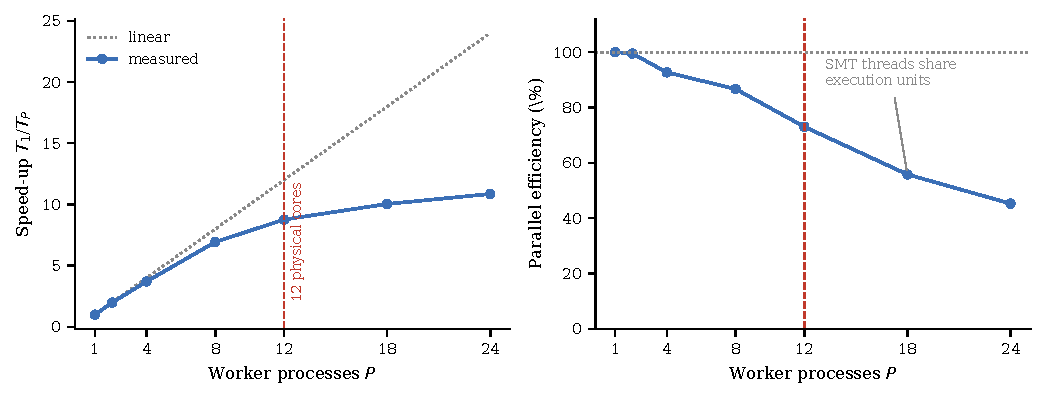
\includegraphics[width=\textwidth]{figures/fig_scaling.pdf}
\caption{Strong scaling of the model-selection workload on the reference
         machine, $72$ independent units, BLAS pinned to one thread per worker.
         Scaling is near-linear to $8$ workers ($6.9\times$, $87\%$ efficiency)
         and the knee falls at $12$, the physical core count. Beyond it the
         additional workers occupy SMT siblings that share execution units with
         an already-saturated core, so throughput still rises but efficiency
         falls to $56\%$ at $18$ workers and $45\%$ at $24$. The production runs
         use $18$: past the efficiency knee, but chosen for wall time on an
         otherwise idle machine. The efficiency figure is not a curiosity: at
         $56\%$, the clustering stage costs $3.6$~h rather than the $2.0$~h that
         dividing its serial cost by $18$ would suggest.}
\label{fig:scaling}
\end{figure}

Figure~\ref{fig:scaling} shows the measured strong-scaling curve. The shape is
the expected one for a compute-bound, memory-light workload on a simultaneous
multithreading processor, and it makes the operating point explicit: $18$
workers buy a $10.0\times$ speed-up over serial execution, while $12$ would give
$8.8\times$ at much better efficiency. Neither choice is a contribution; the
point of measuring is that the default of one worker per hardware thread is not
obviously right, and here it is not.

\subsection{Measured cost}

\begin{table}[h]
\centering
\caption{Wall-clock cost at $m = 1000$ on an AMD Ryzen~9 9900X (12~cores,
         24~threads, $46$~GiB) with $18$ workers. The evidence differs by row
         and is stated rather than blurred: the fidelity stage is instrumented;
         synthesis is the interval over which its $1.44 \times 10^{5}$ outputs
         were written, so it includes any idle time inside that interval; the
         clustering stage was not instrumented, so its entry is a measurement
         on a uniform random sample of $3000$ of its $1.44 \times 10^{5}$ inputs,
         run at the same worker count, scaled to the full set; this is consistent
         with the loose upper bound of $5.6$~h implied by its output
         timestamps.}
\label{tab:cost}
\small
\begin{tabular}{llrr}
\toprule
Stage & Evidence & Wall time & Unit cost \\
\midrule
Synthesis ($1.44 \times 10^{5}$ datasets) & write interval & $1.24$ h & $31$ ms/dataset \\
Clustering ($7.2 \times 10^{5}$ pairs)    & sampled        & $\approx 3.6$ h & $\approx 18$ ms/pair \\
Fidelity ($1.15 \times 10^{7}$ fits)      & instrumented   & $4.44$ h & $1.4$ ms/fit \\
\midrule
Total & & $\approx 9.3$ h & \\
\bottomrule
\end{tabular}
\end{table}

The synthetic datasets occupy $21$~GB as uncompressed Parquet. Cost is linear in
$m$: the same design at $m = 100$ completes in about a tenth of the time and
reproduces every estimate reported here to within $0.025$, so the larger run
buys precision rather than a change in any conclusion.


\end{appendices}
\DIFdelbegin %DIFDELCMD < 

%DIFDELCMD < \bibliography{refs}
%DIFDELCMD < %%%
\DIFdelend 

\end{document}
